\documentclass[12pt]{article}

\usepackage{tgtermes}
\usepackage{epsf}
\usepackage{epstopdf}
\usepackage{amsmath}
\usepackage{graphicx}
\usepackage{booktabs}
\usepackage[colorlinks=true,linkcolor=blue,citecolor=blue]{hyperref}
\usepackage{dcolumn}
\usepackage{amsmath, amsthm, amssymb}
\usepackage{mwe}
\usepackage{url}
%\usepackage{harvard}
\usepackage{fancyheadings}
\usepackage{longtable}
\usepackage{authblk}
\usepackage{setspace}
%\usepackage[nomarkers]{endfloat}
\usepackage{float}
\usepackage{bbm}
%\usepackage{titling}
\usepackage{subcaption}
\usepackage{algorithm}
\usepackage{algorithmic}
\usepackage{import}
\usepackage[backend=biber,style=authoryear,
sorting=ynt,citestyle=authoryear]{biblatex}
\addbibresource{papercitations.bib}
%\usepackage[nomarkers,nofiglist,notablist]{endfloat}
\usepackage{subcaption}
\usepackage{caption}

\onehalfspacing
\textwidth 6.5in \oddsidemargin 0in \evensidemargin -0.6in
\textheight 8.5in \topmargin -0.2in

\newcolumntype{L}[1]{>{\raggedright\let\newline\\
		\arraybackslash\hspace{0pt}}m{#1}}
\newcolumntype{C}[1]{>{\centering\let\newline\\
		\arraybackslash\hspace{0pt}}m{#1}}
\newcolumntype{R}[1]{>{\raggedleft\let\newline\\
		\arraybackslash\hspace{0pt}}m{#1}}
\newcolumntype{P}[1]{>{\raggedright\tabularxbackslash}p{#1}}

\newtheorem{theorem}{Theorem}[section]
\newtheorem{corollary}[theorem]{Corollary}
\newtheorem{proposition}[theorem]{Proposition}
\newtheorem{lemma}[theorem]{Lemma}

\captionsetup{justification=centering,singlelinecheck=false}


\newcommand{\xsub}[1]{%
	\mbox{\scriptsize\begin{tabular}{@{}c@{}}#1\end{tabular}}%
}

%\renewcommand{\thetable}{\Roman{table}}

\begin{document}
	
	
	
	
	\linespread{1.2}\title{\vspace{-0.5in} Does Hospital Leadership Matter?\\ \large Evidence from Pay-for-Performance Incentives} 
	
	\date{\today}
	
	\author{\vspace{10mm}Hanna Glenn\footnote{Department of Economics, Emory University, 1602 Fishburne Drive, Atlanta, GA 30322, hanna.glenn@emory.edu.} }
	
	\maketitle
	%\setlength{\droptitle}{-10pt}
	
	\vspace{-0.2in}
	
	\singlespacing\maketitle


 \vspace{3mm}
	
    \begin{abstract}
		{\small
         One determinant of firm behaviors and performance is the type of management leading the firm. Characteristics such as age, gender, and background are correlated with employee wages, decisions of mergers and acquisitions, and other firm outcomes. In this paper, I investigate this topic in the context of hospital executive teams. Specifically, I estimate the effect of clinically trained executives on hospital quality. I leverage pay-for-performance policies that changed quality incentives for hospitals in the US in 2012, and estimate the difference in readmission and mortality rates for nonprofit hospitals with and without clinically trained executives. I find that clinically trained executives do not improve quality as much as executive teams without clinically trained executives. This difference is not driven by a change in patient complexity, but may be driven by preferences towards profit vs. patient welfare. Further, clinically trained executives are not just a signal of underlying hospital incentives, but manage the hospital differently. 
		} 
	\end{abstract}
	
	
	
	
	\vspace{0.8in}
	
	\noindent Keywords: 
	
	\noindent JEL Codes: 
	
	\onehalfspacing
	
	\newpage

    Broadly, firm leader characteristics such as gender, age, and background have been shown to be correlated with financial performance and behaviors such as employee diversity, wages, aggressiveness in mergers and acquisitions, and other corporate strategies. I consider this topic in the context of hospital quality under executives with differing backgrounds: some with training as a medical doctor and some without. Physicians can bring a unique combination of clinical and administration expertise, and they have insights that can potentially benefit their employees and lead to better quality (\cite{Stajduhar_2023}, \cite{Ahmed_2022}). However, hiring physician executives can also be controversial, as physicians are not always adequately trained in business management, which can lead to poor business practices and lower quality (\cite{HarvardBusinessReview2018}). 

    In this paper, I estimate how having clinically trained executives in leadership affects quality of care in hospitals. I scrape executive team names and titles from publicly available Tax Form 990s, filled out by nonprofit firms in the US. Combining this with publicly available hospital characteristics, I construct a novel data set of nonprofit hospitals from 2010-2014 containing information on both executive team characteristics and quality metrics. While limited to nonprofit hospitals due to data availability, this sample is a very important driver of health care in the US. Private nonprofit hospitals make up 50\% of all hospitals in the US, and staff, on average, 207 beds. For comparison, for-profits make up 36\% of hospitals and staff 107 beds (\cite{ASPE_2023}). Therefore, the behavior of these hospitals directly affects health care consumers in the US. 
    
    The non-random selection of leaders makes it difficult to interpret any direct comparison of differing executive teams as causal. Therefore, I leverage an exogenous shock to hospital incentives, pay-for-performance policies enacted in the US in 2012, and compare the change in readmission and mortality rates of executive teams with and without clinical executives. Under the assumption that the two types of teams would have had similar trends in readmission and mortality rates absent the incentive change, I find that executive teams with clinical executives on average do not improve quality as much as executive teams without clinical executives. While both types of hospital leadership teams decrease readmission rates after the policy change, those without clinical executives decrease readmissions at a faster rate than those with clinical executives. 
    
    Having found that hospital leadership does, in fact, matter to hospital behavior, I investigate several mechanisms that might contribute to this difference. First, the more drastic decrease in readmissions by non-clinical teams is not driven by decreasing average patient complexity. Further, comparing each type of leadership team with for-profit hospitals reveals that the absence of clinical executives leads a nonprofit hospital to respond more similarly to a for-profit hospital than nonprofits with clinical executives. That is, having clinical training on a leadership team leads a hospital to act less profit-driven than their general training counterparts. Finally, I show that changes in a hospital's propensity to hire a clinical executive are not correlated with the pay-for-performance policies. Thus, I exploit such changes in leadership teams to decompose the effect of clinical executives into signaling (clinical executives signal underlying hospital preferences), or managing (clinical executives manage the hospital differently). I find that the entire difference in response is driven by a managing effect. 

    Many researchers have documented a correlation between executive characteristics and firm performance, starting with \citeauthor{bertrand2003managing} (\citeyear{bertrand2003managing}), who show that manager fixed effects are an important driver of many firm behaviors and decisions. Female board members are associated with better oversight and more women executives (\cite{matsa2011chipping}; \cite{adams2009women}), but are negatively correlated with firm value (\cite{ahern2012changing}). Having more female executives is correlated with female employee wages and corporate strategies (\cite{flabbi2019female}; \cite{matsa2013female}); young male CEOs tend to be more aggressive in mergers and acquisitions, while those with military experience are less aggressive (\cite{levi2010deal}; \cite{benmelech2015military}); CEOs with general ability tend to receive higher pay and perform better (\cite{kaplan2012ceo}; \cite{custodio2013generalists}; \cite{adams2018director}; \cite{frydman2019rising}). Finally, Chief Diversity Officers are not found to have any effect on hiring more diversely in universities (\cite{bradley2022impact}). 
    
    Due to data limitations, many of these studies focus on large, publicly traded firms in the US. \citeauthor{brickley2010board} (\citeyear{brickley2010board}) have the only study to my knowledge in the US nonprofit context considering hospital board of directors. Using exogenous variation in expected Medicare profits, the authors find that having an internal board of directors increases CEO compensation, and having physician board members decreases public donations (\cite{brickley2010board}). Additionally, two studies focus on hospital performance in other countries. \citeauthor{janke2019impact} (\citeyear{janke2019impact}) use data from England to study whether CEOs affect hospital production, and find no association (\cite{janke2019impact}). However, \citeauthor{otero2022managers} (\citeyear{otero2022managers}) investigate the role of CEOs in public hospitals in Chile, and finds an 8\% decrease in mortality rates for hospitals with top managers. Further, a major contributor of this quality improvement is the exodus of older physicians as CEOs (\cite{otero2022managers}). I contribute to our knowledge of how executive team characteristics affect firm behaviors by (1) considering the important setting of nonprofit hospitals, which serve the majority of patients in the US, (2) considering a unique and relevant executive characteristic, and (3) observing firm behavior in the presence of an exogenous incentive change. 

    Additionally, I contribute to our understanding of how providers respond to pay-for-performance incentives in health care. The most in depth study of how hospitals respond to the Hospital Readmissions Reduction Program, one of the two large pay-for-performance initiatives, is \citeauthor{gupta2021impacts} (\citeyear{gupta2021impacts}). This study finds that hospitals decreased readmissions by 5\% and mortality rates by 2\% on average as a result of the program, confirming prior studies (\cite{mellor2017does}; \cite{ziedan2018essays}; \cite{ody2019decreases}; \cite{gupta2021impacts}). Around 40\% of the decrease in readmissions is due to selective patient practices. Further, market concentration and hospital systems play a large role in how hospitals respond to the program (\cite{kunz2024assessing}). Research on the other large pay-for-performance initiative, the Hospital Value Based Purchasing Program, generally finds that the program had no effect on underlying hospital quality (\cite{us2015hospital}; \cite{norton2018moneyball}; \cite{friedson2019so}). This paper contributes to our understanding of how characteristics of hospitals affect response to pay-for-performance incentives.

    \section{Setting and Data}

    \subsection{Nonprofit Hospital Executives}

    Nonprofit firms in the US differ from for-profits mainly in that for-profit firms distribute revenue to stakeholders, while nonprofits reinvest profit back into the firm. Hospitals are governed by a board of directors, whose role is to set broad goals and strategies, and provide general oversight. The board selects executives, the highest level of management of a firm, to carry out day-to-day operations. An executive team usually consists of at least a Chief Executive Officer (CEO) and Chief Financial Officer (CFO), but there is variation in how firms organize executive teams. Some hospital executives specialize in health care settings by earning a degree in health care management, or an MBA specific to health care. There are executive positions that are often filled by someone with clinical training, such as a Chief Medical Officer (CMO), but medical doctors can pursue other top managerial positions as well such as CEO or president. While some doctors earn additional degrees before stepping into an executive role, this is not a necessary condition to becoming a physician executive. 

    Hospital executive teams are understudied partly due to the inaccessibility of granular data. I construct a novel data set of nonprofit hospitals in the US which contains names, titles, and positions of all board members and executives tied to the hospital from 2009-2015. I gather this data from publicly available Tax Form 990s, which every sufficiently large nonprofit files each year in the US. To my knowledge, this is the first large scale gathering of executive names from these forms.\footnote{\citeauthor{brickley2010board} (\citeyear{brickley2010board}) collects compensation data for a select number of hospitals.} 

    All tax-exempt organizations in the US are required to file a Form 990 with Internal Revenue Services (IRS) each year. There are different types of forms, but any organization grossing over \$200,000 must file the most extensive Form 990. Sections of this form include a statement of revenue, statement of functional expenses, a balance sheet, and, as used in this project, a list of all key employees, executives, and board members. Each firm is required to report the name and title, average hours per week, position, and compensation of their board members and executives. 

    The historical tax forms are housed by ProPublica.\footnote{https://projects.propublica.org/not-for-profits/} I use the NonProfit Explorer API to extract Employee Identification Numbers (EIN) of firms with a hospital National Taxonomy of Exempt Entities (NTEE) code. After filtering out associations and specialty hospitals, there are approximately 3,000 EINs. Linking these EINs to other hospital information is crucial to the analysis, but no crosswalk from EIN to other hospital identifiers is publicly available. I therefore rely on matching by location and name of hospital in both the tax forms and American Hospital Association (AHA) data. In the AHA data, I limit to general hospitals. Then, I confidently match 1200 EINs to an AHA identification number based on exact name matches within the same state.\footnote{I assess the observable differences between matched and non-matched hospitals in Appendix \ref{app:matched}, and conclude that the samples are overall similar apart from an under-sampling of hospitals that belong to systems.}
    
    For each of the matched EINs, I extract web URLs to Form 990 PDFs for each year. I use an algorithm to download these locally and use optical character recognition (OCR) text extraction methods to scrape the relevant section of the PDF, which is titled ``Officers, Directors, Trustees, Key Employees, and Highest Compensated Employees". Finally, I use string cleaning methods to identify all names and positions under each EIN, year. With each name, I extract titles indicating clinical training: MD, Dr., or DO. Using OCR extraction can be unreliable in cases where the text on the form is handwritten or small. Therefore, for observations that are missing after the initial extraction, I manually record names, positions, and titles. As I limit the sample to hospitals who have text information in every year, I limit the years to 2010-2014 to retain more hospitals. This yields 852 nonprofit hospitals that are matched to AHA data, and with complete text information in each year. 

    Finally, I seek to (1) verify clinical training of those who claim to be doctors, and (2) obtain additional information about clinically trained executives. Thus, I match each name with the National Plan and Provider Enumeration System (NPPES) database of all registered physicians. For any person who has a doctor title and uniquely matches the NPPES data, I record their National Provider Identifier (NPI) number. For anyone who has a doctor title and no matches, no doctor title and matches, or a doctor title and multiple matches, I use information on location and hospital name to manually match NPI numbers of those who did have clinical training. I present a table of means for various characteristics of doctor executives in the data in Table \ref{doc_sumstats}. In total, there are 813 doctor executives. On average, they are 52 years old, and 11\% of them are female. While it is more likely they are a Chief Medical Officer than a Chief Executive Officer, still less than a third are CMOs. The most common specialty is internal medicine. 

    \import{Tables}{doc_exec_stats_tab.tex}

    For the purposes of this paper, I focus on executive teams as a whole instead of specific positions. The main reason for this is because the organization of teams varies so drastically across hospitals. It is not uncommon for two hospitals to have the same position but the tasks performed are drastically different, or to have two distinct positions that essentially perform the same tasks. I drop anyone who is solely a board member, and focus on those who have executive in their title, or are labeled as a president or vice president of a department. I create various hospital-level characterizations based on their executive team, such as the existence of a clinically trained executive, the number of clinically trained executives, the number of total executives, and whether the hospital has a Chief Medical Officer. For the main analysis, I limit to hospitals who either always have a clinical executive or never have a clinical executive over the course of the sample in order to have a clean comparison.
  
    \subsection{Pay-for-Performance Policies Targeting Readmission and Mortality Rates}\label{sec:hrrp}

    Two programs were passed as part of the Affordable Care Act that focused on pay-for-performance incentives for hospitals: the Hospital Readmissions Reduction Program (HRRP), and the Hospital Value Based Purchasing Program (HVBP). HRRP focused on penalizing hospitals with poor quality, and HVBP focused on rewarding hospitals with high quality or show improvement in quality. 

    In October 2011, the Center for Medicare and Medicaid Services (CMS) released a set of rules under HRRP mandating penalties for hospitals with above average readmission rates. The goal of HRRP is to lower readmissions through better care coordination, less initial stay complications, and better post-care instructions. Beginning in October 2012, hospitals with higher readmission rates than the national average in pneumonia, heart failure, or AMI (after adjusting for demographic characteristics) receive a fixed lower reimbursement rate for all Medicare patients seen in their hospital. In 2015, CMS also included chronic obstructive pulmonary disease, coronary artery bypass graft surgery, and elective primary total hip arthroplasty and/or total knee arthroplasty as conditions which go into the penalty calculation (\cite{CMS}). 
    
    Penalties are given in the form of a fixed rate reduction of 1-3\% for every Medicare patient regardless of the condition. Further, CMS does not distinguish a necessary readmission from an avoidable readmission; any repeat hospital visit is included in the penalty calculation. Excess readmission rates are calculated using a rolling look-back period of 3 years to determine whether the hospital is penalized. Therefore, hospitals had incentive to react immediately once details of the program were announced in October of 2011. 

    The HVBP Program instead rewards hospitals with high quality or significant improvement in quality. Specifically, CMS deducts Medicare payments by 2\% from all eligible hospitals, collects this sum, and divides it among the rewarded hospitals. Several quality and cost measures surrounding safety, efficiency, cost reductions, clinical outcomes, and community engagement are combined to create a single score metric for each hospital. Hospitals are then compared to the average and are rewarded for being above average quality or for showing improvement (\cite{CMS_2023}). 

    I focus on outcomes of readmission and mortality rates, which are publicly available at the hospital-condition level in CMS Hospital Compare. I combine rates for pneumonia, AMI, and heart failure (the relevant HRRP conditions) into a weighted average based on the number of patients in each condition. Additionally, I include several relevant hospital characteristics from the AHA survey: number of beds, and whether the hospital is an academic medical center, is physician owned, or is system affiliated. Additionally, case mix index, a measure of overall patient complexity, comes from the CMS Case Mix Index files. Whether the hospital was penalized under HRRP or received payments under HVBP is found in the HCRIS data. 

	\subsection{Summary Statistics}\label{sec:data}

    The hospitals in my sample are limited to general nonprofit hospitals with executive team information in each year (2010-2014) and a link from EIN to AHA ID. In Table \ref{tab:sumstats_samples_stable}, I present means of relevant variables for several hospital samples used throughout the paper. First, in column (1), are means for hospitals who ever have a clinical executive at any point in the sample. In column (2) are means for hospitals who have a clinical executive for the entire sample period, and column (3) shows means for hospitals who never have a clinical executive in the sample period. The main analysis compares hospitals in columns (2) and (3), and supplemental analyses leverage hospitals in column (1). 

    \import{Tables}{stable_sample_sumstats.tex}

    Hospitals that never have a clinical executive are smaller, less likely to be an academic medical center, and less likely to be affiliated with a system. Further, they have smaller executive teams on average by 1-2 people, and are less likely to have anyone acting as a CMO.\footnote{Though, they may title the position differently.} Finally, in regards to exposure to pay-for-performance programs, hospitals who never have clinical executives are less likely to receive benefits from the HVBP Program, but seem more similar to hospitals with clinical leadership in terms of penalties from HRRP. 

    Next, I plot weighted average readmission, mortality rates, and patient case mix index across time for different hospital types in Figure \ref{fig:outcomes_graph}. Pay-for-performance incentive change timing is shown as a dotted line in 2012. Average readmission rates trend similarly prior to 2012, and all hospital type exhibit a decrease in readmission after 2012. However, hospitals who consistently have a clinical executive show a slower rate of decrease in raw readmissions. When considering mortality, there is not a drastic change in 2012 for any hospital type, but hospitals who always have a clinical executive continue on an increasing trend in mortality where the other hospitals types remain more flat. Finally, hospitals that never have clinical executives consistently have less complex patients, but there is no notable change in raw case mix index over time.

    \begin{figure}[ht!]
    \centering
        \caption{Outcomes Over Time}
        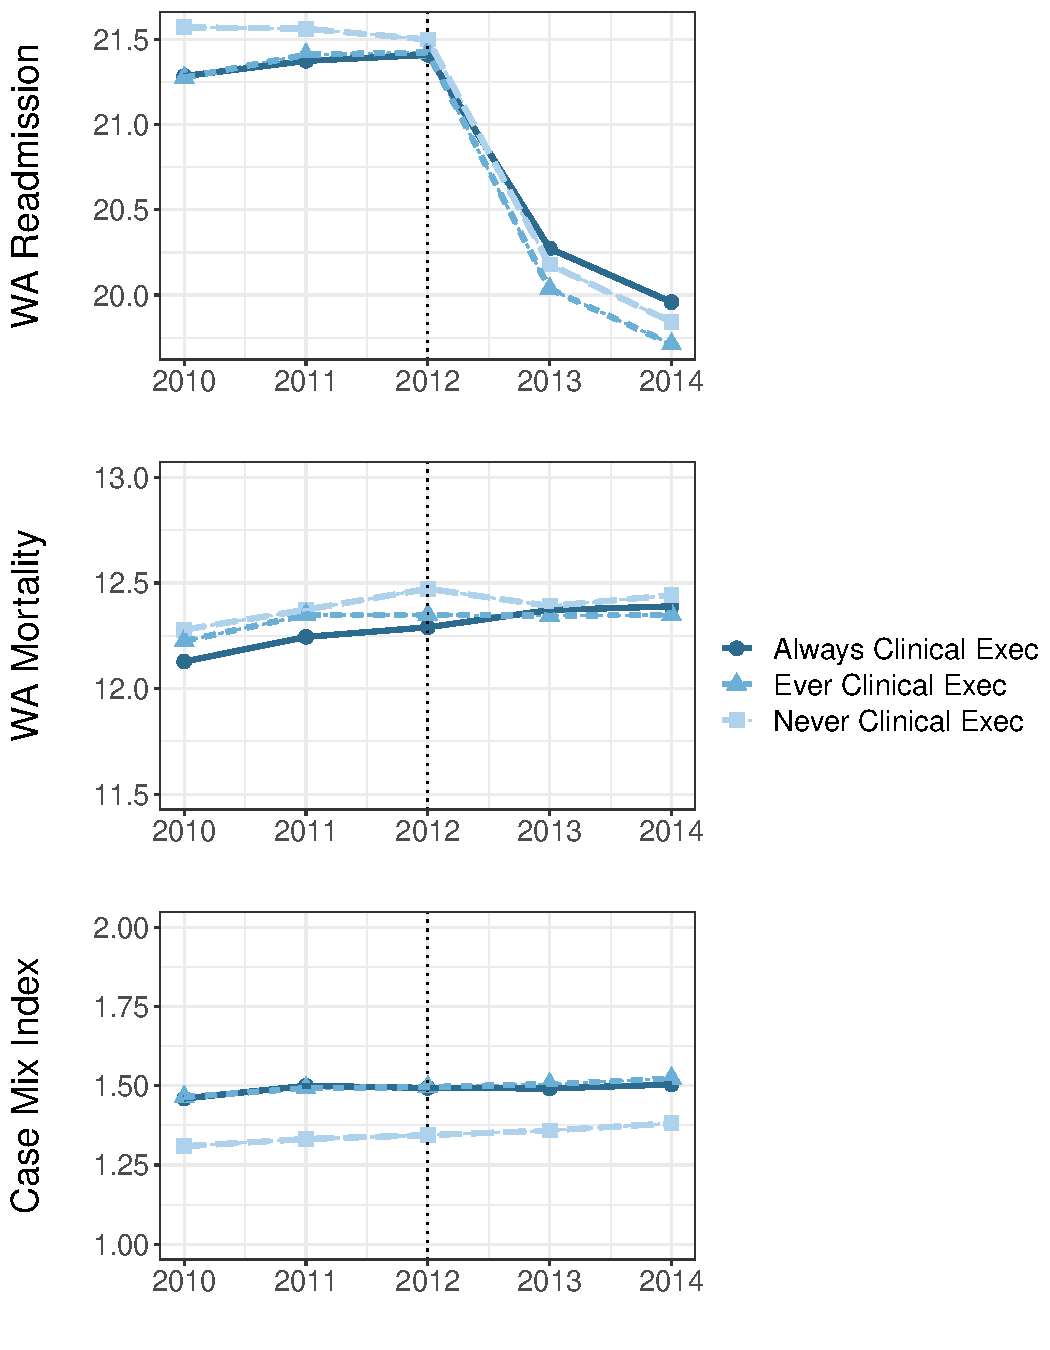
\includegraphics[width=.8\textwidth]{Objects/outcomes_graph.pdf}
        \label{fig:outcomes_graph}
    \end{figure}


    \section{Effect of Executive Clinical Training on Hospital Quality}\label{sec:clinical}

    First, I test empirically whether having clinical training matters in how hospitals change readmission and mortality rates in response to the pay-for-performance policies effective in 2012. For a clean comparison, I limit the sample to hospitals who always have clinical executives or never have clinical executives. That is, these hospitals do not change their propensity to hire a clinical executive during the sample period. Therefore, an important assumption that I make is that this sample selection is not correlated with the program enactment. I investigate this assumption in Section \ref{sec:changes}, and find no evidence that hospitals are more or less likely to change their propensity to hire a clinical executive because of the pay-for-performance programs. 
    
    I estimate a two-way-fixed-effects specification, where the key independent variable is the interaction between having clinically trained executives and post 2012, when the programs began. Importantly, I am not estimating the effect of being penalized. All hospitals had incentive to improve quality in response to the policy change, as penalties and payments are determined by comparing quality among hospitals. Thus, I leverage the timing of the policy change, rather than the policies themselves. However, because of potential differences in quality trends between clinical and non-clinical hospital executive teams even before the policies, I employ a synthetic difference-in-differences estimation strategy (\cite{arkhangelsky2021synthetic}). That is, hospitals in the control group with similar trends in readmission, mortality, and baseline case mix before the programs are more heavily weighted, as well as time periods that balance pre- and post-program outcomes for hospitals without clinical executives. Below is the unweighted specification for clarity, where the identification assumptions are conceptually the same for synthetic difference-in-differences: 

    \begin{equation}
    \label{eq:clinical}
    y_{ht} = \beta \text{ (clinical training x post 2012)}_{ht} + \gamma_{h} + \delta_t + \epsilon_{ht},
    \end{equation}
    

    \noindent where $y_{ht}$ is one of the outcome variables capturing readmission or mortality rates discussed in Section \ref{sec:hrrp}, and $\gamma_h$ and $\delta_t$ are hospital and time fixed effects, respectively. 

    In the unweighted two-way-fixed-effects specification, we have reason to believe that the parallel trends assumption may not hold due to observed differences in characteristics other than the leadership team, as discussed in Section \ref{sec:data}. Once incorporating the weights used in the synthetic differences in differences method, we ensure parallel trends in the outcome variables prior to 2012. Thus, I assume that under the weighted clinical and non-clinical hospital composition, trends would have continued to be parallel absent the incentive change in 2012. A component of this assumption is the implicit assumption that no other event occurred in 2012 correlated with both the outcomes and composition of leadership team. Finally, I assume that there is no anticipation of the policy change before 2012. The rules of the policies were announced in October of 2011, so 2012 was the first full year that hospitals could meaningfully respond to the policies.

    The estimated difference in readmission and mortality rates between hospitals with and without clinical executives are shown in Figure \ref{fig:clinicalsynthdid}. Estimate $\beta$ is represented in the difference in slope after 2012 when pay-for-performance incentives began. Panel \ref{fig:read_synth_clinical} shows the estimated difference in readmission rates, and reveals that non-clinical teams decrease readmissions by .3 (standard error .13) more than clinical teams. This is a relatively small magnitude given an average readmission rate of 21, but reveals a meaningful difference in behavior given that both hospital types significantly decrease readmissions. In panel \ref{fig:mort_synth_clinical}, I show the estimated difference in mortality. While the magnitude of the difference is similar to that for readmission rates, mortality is a noisy measure, and I cannot rule out no difference in mortality response. In Appendix \ref{app:condition}, I show that these results are primarily driven by pneumonia patients.  

     \begin{figure}[ht!]
     \caption{Effect of Clinical Experience on Readmission and Mortality Rates}
     \centering
     \begin{subfigure}[b]{0.45\textwidth}
         \centering
         \caption{Readmission Rate}
         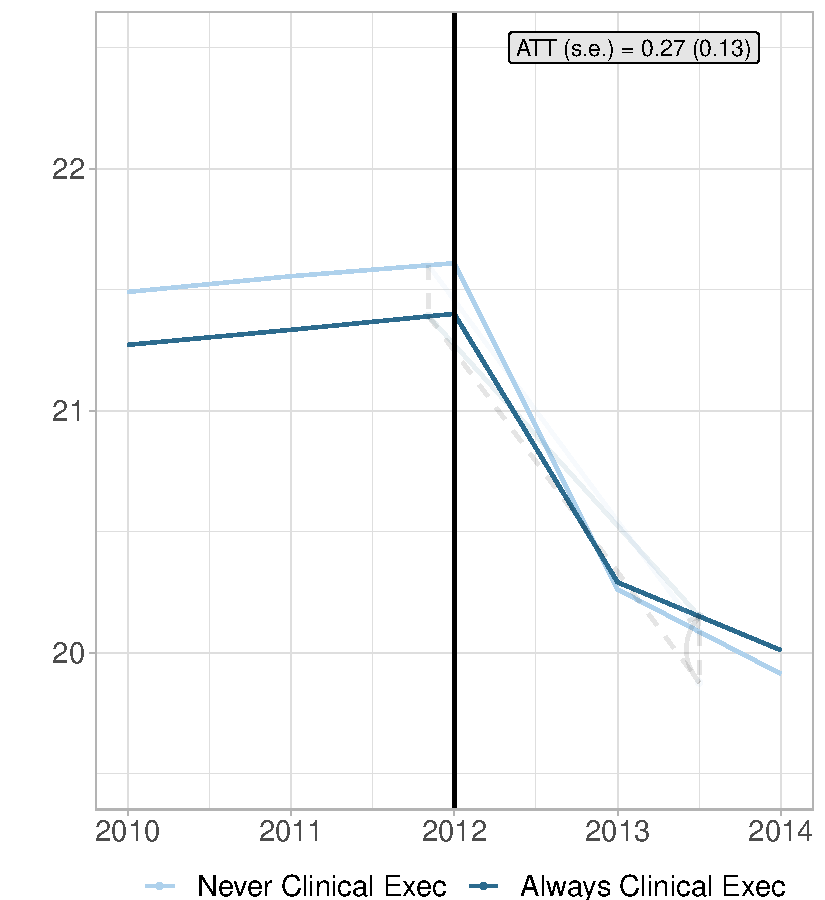
\includegraphics[width=\textwidth]{Objects/read_md_nomd_synth_graph.pdf}
         \label{fig:read_synth_clinical}
     \end{subfigure}
     \hfill
     \begin{subfigure}[b]{0.45\textwidth}
         \centering
         \caption{Mortality Rate}
         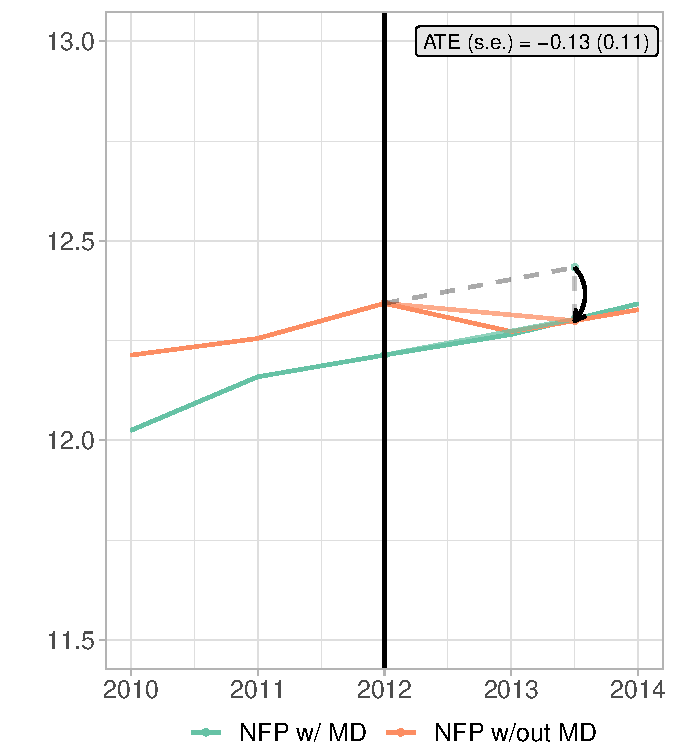
\includegraphics[width=\textwidth]{Objects/mort_md_nomd_synth_graph.pdf}
         \label{fig:mort_synth_clinical}
     \end{subfigure}
        \label{fig:clinicalsynthdid}
    \end{figure}

    Additionally, I estimate the intensive margin of clinical leadership: whether the fraction of clinical executives on the team affects quality. I bin the fraction of clinical executives into less than a quarter or more than a quarter and less than one half.\footnote{Less than .5\% of hospitals have greater than 50\% clinical executives on the team.} Then, I estimate:

    \begin{equation}
    \label{eq:clinical_continuous_onefourth}
    y_{ht} = \beta \left(\mathbbm{1}\{0 < \rho \leq .25\}\text{ x post 2012}\right)_{ht} + \gamma_{h} + \delta_t + \epsilon_{ht}, \text{ and}
    \end{equation}
    \begin{equation}
    \label{eq:clinical_continuous_onehalf}
    y_{ht} = \beta \left(\mathbbm{1}\{.25 < \rho \leq .5\}\text{ x post 2012}\right)_{ht} + \gamma_{h} + \delta_t + \epsilon_{ht},
    \end{equation}

    \noindent where $\rho$ is the fraction of clinical executives on hospital $h$'s executive team, and $\gamma$ and $\delta$ are fixed effects as defined in Equation \ref{eq:clinical}. 

    I show the results of this estimation with readmission rates as the outcome in Figure \ref{fig:cont_clinicalsynthdid}. In panel \ref{fig:onefourth_read_synth_clinical}, the estimation compares executive teams with no clinical experience to those with up to 25\% of the team having clinical experience. The average treatment effect is .04 and not statistically significant. Thus, there is no significant difference in how these types of teams respond to the incentive change. In panel \ref{fig:onehalf_read_synth_clinical}, I compare hospitals with no clinically trained executives over the course of the sample to hospitals with over a quarter of their team having clinical training. While these hospitals have parallel pre-trends, hospitals without clinically trained executives decrease readmissions by .64 (standard error .33) more than hospitals with clinically trained executives. Thus, the readmission rate response is fully driven by having a higher proportion of clinical executives relative to no clinical executives.

    \begin{figure}[ht!]
     \caption{Effect of Clinical Experience on Readmission Rates, Binned Treatment}
     \centering
     \begin{subfigure}[b]{0.45\textwidth}
         \centering
         \caption{$0 < \rho \leq .25$}
         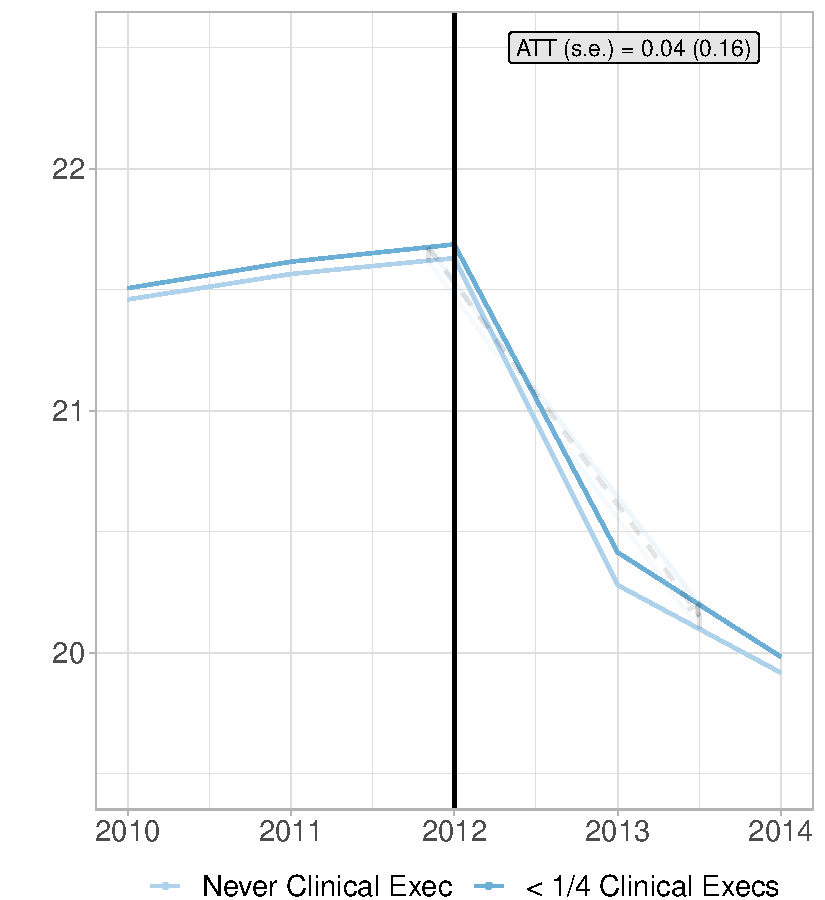
\includegraphics[width=\textwidth]{Objects/cont_onefourthread_md_nomd_synth_graph.pdf}
         \label{fig:onefourth_read_synth_clinical}
     \end{subfigure}
     \hfill
     \begin{subfigure}[b]{0.45\textwidth}
         \centering
         \caption{$.25 < \rho \leq .5$}
         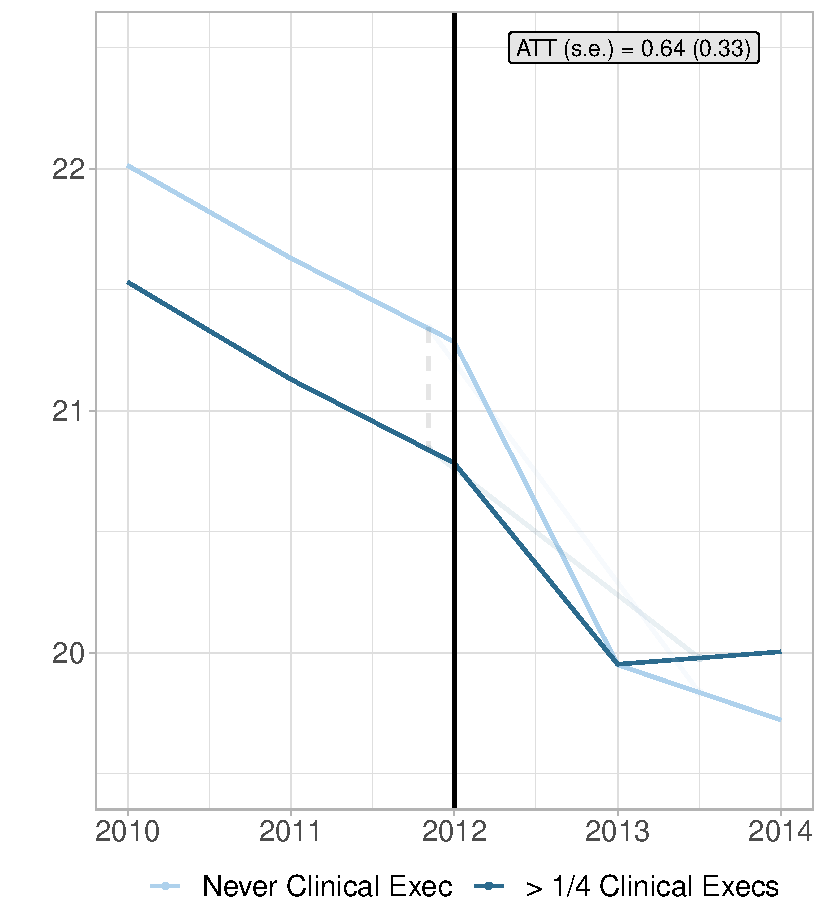
\includegraphics[width=\textwidth]{Objects/cont_onehalfread_md_nomd_synth_graph.pdf}
         \label{fig:onehalf_read_synth_clinical}
     \end{subfigure}
        \label{fig:cont_clinicalsynthdid}
    \end{figure}

    Any potential difference in mortality rate response also seems to be driven by executive teams with over a quarter of the executives having clinical experience, as shown in Figure \ref{fig:cont_clinicalsynthdid_mort}. However, the standard errors of this estimation are high, potentially due to the noisiness in the mortality measure. The magnitude of the estimate in panel $\ref{fig:onefourth_mort_synth_clinical}$ is .07, so I can rule out differential responses by teams with less than a quarter of clinical executives. Taking the readmission and mortality rate results together, the effect of having clinical leadership on quality after an incentive change depends on having a sufficient proportion of the team with clinical training. 


    \begin{figure}[ht!]
     \caption{Effect of Clinical Experience on Mortality Rates, Binned Treatment}
     \centering
     \begin{subfigure}[b]{0.45\textwidth}
         \centering
         \caption{$0 < \rho \leq .25$}
         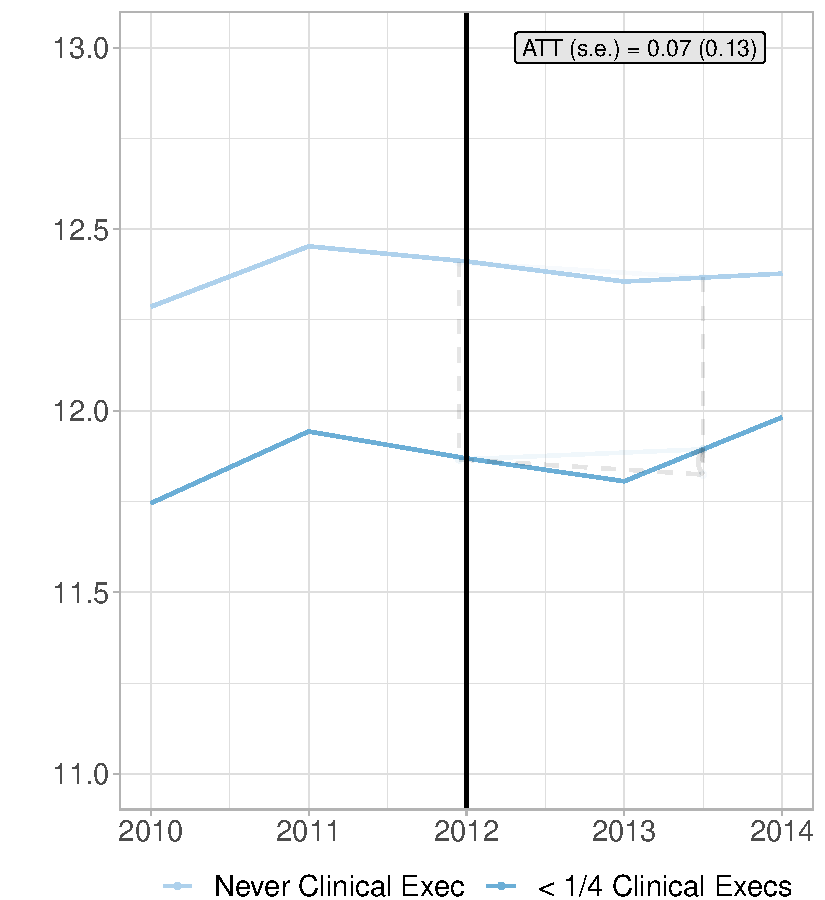
\includegraphics[width=\textwidth]{Objects/cont_onefourthmort_md_nomd_synth_graph.pdf}
         \label{fig:onefourth_mort_synth_clinical}
     \end{subfigure}
     \hfill
     \begin{subfigure}[b]{0.45\textwidth}
         \centering
         \caption{$.25 < \rho \leq .5$}
         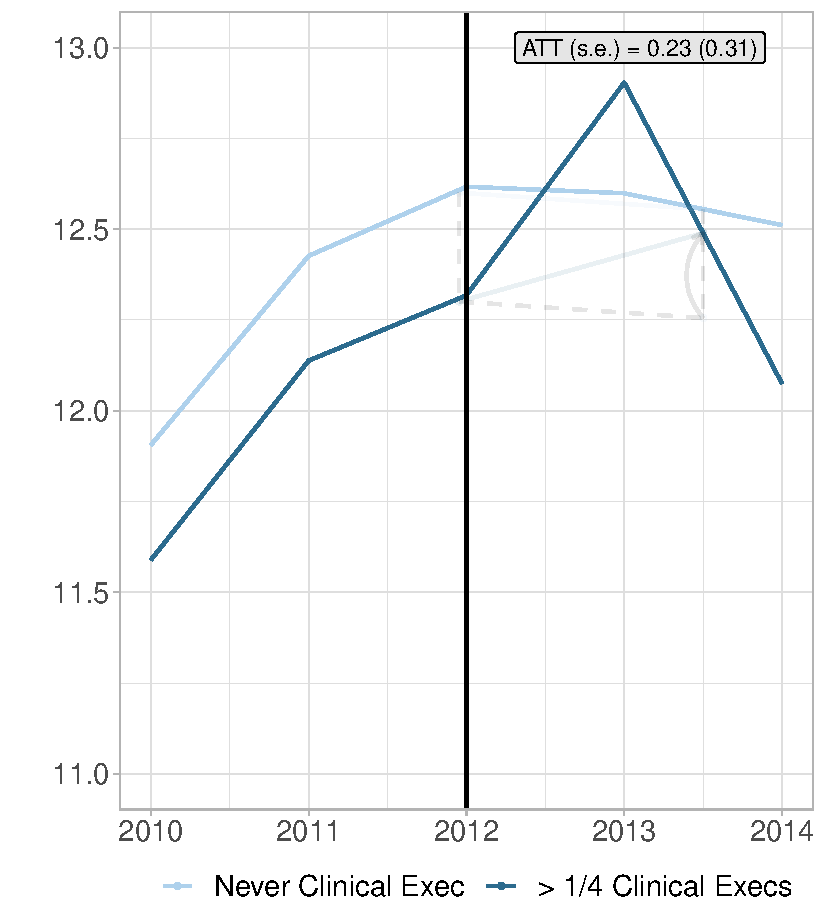
\includegraphics[width=\textwidth]{Objects/cont_onehalfmort_md_nomd_synth_graph.pdf}
         \label{fig:onehalf_mort_synth_clinical}
     \end{subfigure}
        \label{fig:cont_clinicalsynthdid_mort}
    \end{figure}

    

    \section{Selective Patient Practices}

    A method hospitals have been shown to employ in order to decrease readmission rates is being more selective with which patients to admit to the hospital (\cite{gupta2021impacts}). One hypothesis behind a more drastic quality decrease by non-clinical teams is that they may be more willing to participate in such practices, while executives with clinical training prioritize care for all types of patients. 

    To test this, I employ case mix index as the outcome in specification \ref{eq:clinical} to determine whether one type of hospital differentially changes patient composition after pay-for-performance incentives, where the same identification assumptions hold. I present the estimated difference in Figure \ref{fig:main_cmi_clinical}, comparing hospitals that never have a clinical executive to hospitals that always have a clinical executive. Neither type of hospital drastically changes case mix index after the incentive change, and there is no estimated differential response in complexity of patients seen in the hospital. Thus, the estimated difference in readmission rate response between clinical and non-clinical executives is not due to differentially changing case mix. 

    \begin{figure}[ht!]
        \centering
        \caption{Effect of Clinical Executive on Cases Mix Index}
        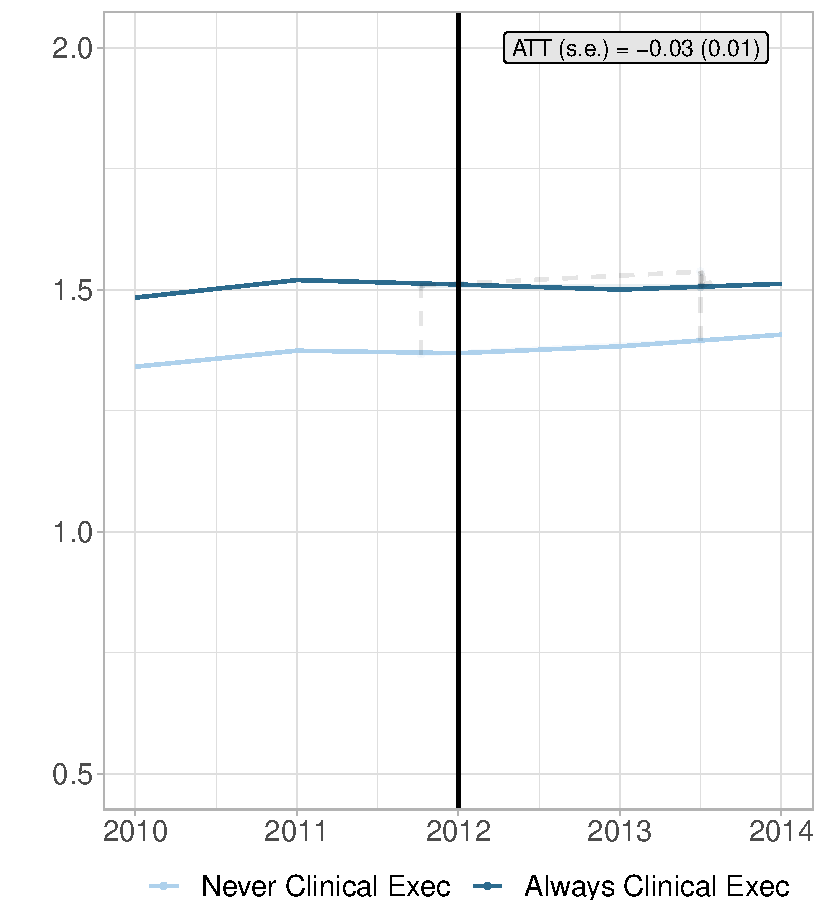
\includegraphics[width=0.5\textwidth]{Objects/cmi_md_nomd_synth_graph.pdf}
        \label{fig:main_cmi_clinical}
    \end{figure}

    \section{Internal Medicine vs. Other Specialties}

    While most doctors still take a hippocratic oath to care for patients with integrity and compassion, doctors with training in certain specialties may be more equipped to improve care for patients with the specific conditions relevant in this context. Specifically, a pulmonologist typically treats pneumonia, and a cardiologist typically treats heart failure and heart attack patients, which are the three conditions considered in the HRRP penalties. Both of these specialties are under the umbrella of internal medicine. My physician specialty information does not get more granular than internal medicine as a specialty. Thus, I estimate the difference in response between 


    \section{Are Clinical Executives Less Profit Driven?}\label{sec:forprofit}

    Another hypothesis that could explain the differential response due to clinical leadership is how profit-driven a clinician is compared to other training backgrounds. To demonstrate this, consider hospital behavior under the enactment of pay-for-performance policies, where hospitals face a trade-off between profit and societal benefit. Pay-for-performance incentives essentially incorporate quality directly into a hospital's profit function (\cite{dranove2011health}), whereas a fee-for-service system only incentivizes quantity. A hospital that places all value on profit will only care about quality when it enters into the profit function, and therefore will respond more drastically to pay-for-performance than a hospital who already cared about quality through societal benefit before the incentives.\footnote{I present the theoretical model and mathematical results in Appendix \ref{sec:model}.} Therefore, observing hospital responses to pay-for-performance incentives reveals information about their underlying preferences.  

    I merge all general for-profit hospitals in the AHA data to the sample of nonprofit hospitals. Then, I compare readmission and mortality rates of always clinical executives and never clinical executives to for-profit hospitals after the incentive change. Ideally, I would also have leadership heterogeneity information for for-profit hospitals, but this data does not exist publicly. However, on average, for-profit hospitals have revealed through their ownership status that they more heavily weigh profit. Thus, comparing different executive team behavior to for-profit behavior helps reveal how profit driven certain leadership teams are. Thus, I estimate

    \begin{equation}
    \label{eq:forprofit}
    y_{ht} = \beta \text{ (for-profit x post 2012)}_{ht} + \gamma_{h} + \delta_t + \epsilon_{ht}
    \end{equation}

    \noindent for two subsets of data. First, I limit only to for-profits and nonprofits with clinically trained executives. Second, I limit to for-profits and nonprofits without clinically trained executives. Thus, $\beta$ represents the effect of being for-profit compared to being nonprofit with a certain leadership team type. I show summary statistics of relevant variables for for-profit hospitals in Appendix \ref{app:sumstats}. Again, I employ a synthetic difference-in-differences strategy to rely less heavily on a strong parallel trends assumption for different types of hospitals. 

    The identification assumptions I make here are largely similar to those in Section \ref{sec:clinical}, only now incorporate for-profit hospitals. First, I assume that, absent the change in incentives, for-profits and the relevant comparison group would have had parallel trends in outcomes. Second, I assume that the stability of nonprofit leadership teams is not correlated with the 2012 policy changes. I explore this assumption in Section \ref{sec:sig_man}. I also assume that there is no anticipation of the policy changes prior to 2012, which is reasonable as the rules of the policies were announced in October of 2011. Finally, I assume no other changes correlated with both hospital type (for-profit, nonprofit with and without clinically trained executives) and quality occurred in conjunction with the 2012 pay-for-performance policies.

     \begin{figure}[ht!]
     \caption{Comparison to For-Profit: Readmission}
     \centering
     \begin{subfigure}[b]{0.45\textwidth}
         \centering
         \caption{For-Profit and Always Clinical Exec}
         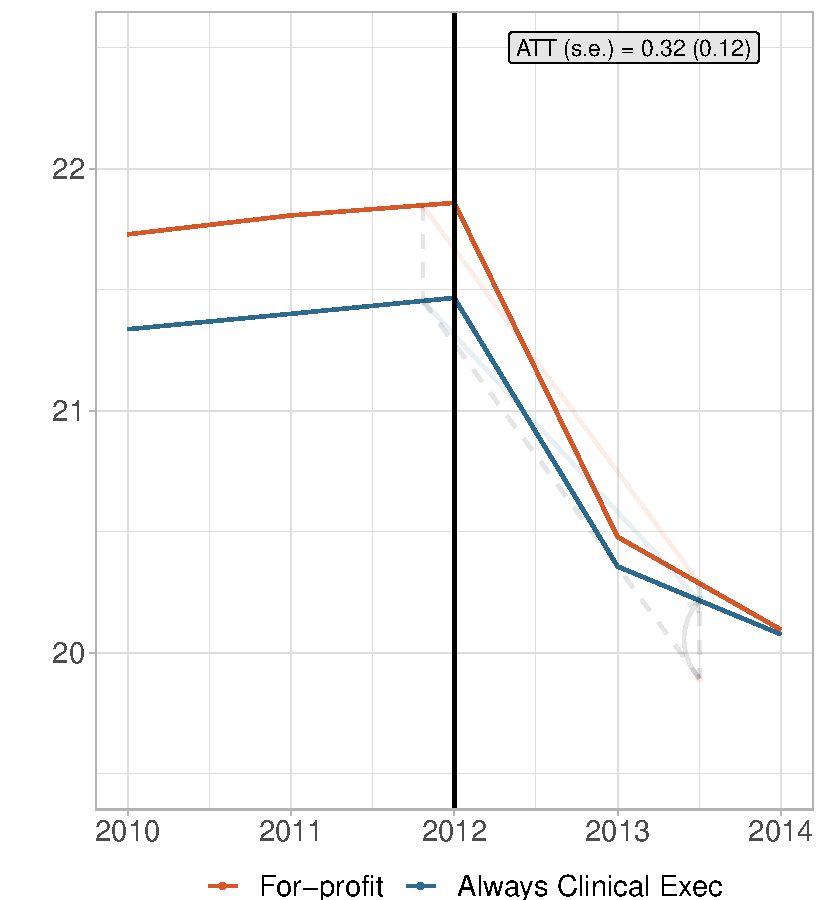
\includegraphics[width=\textwidth]{Objects/fp_read_md_synth_graph.pdf}
         \label{fig:read_synth_plotb}
     \end{subfigure}%
     \vspace{5mm}
     \hfill
     \begin{subfigure}[b]{0.45\textwidth}
         \centering
         \caption{For-Profit and Never Clinical Exec}
         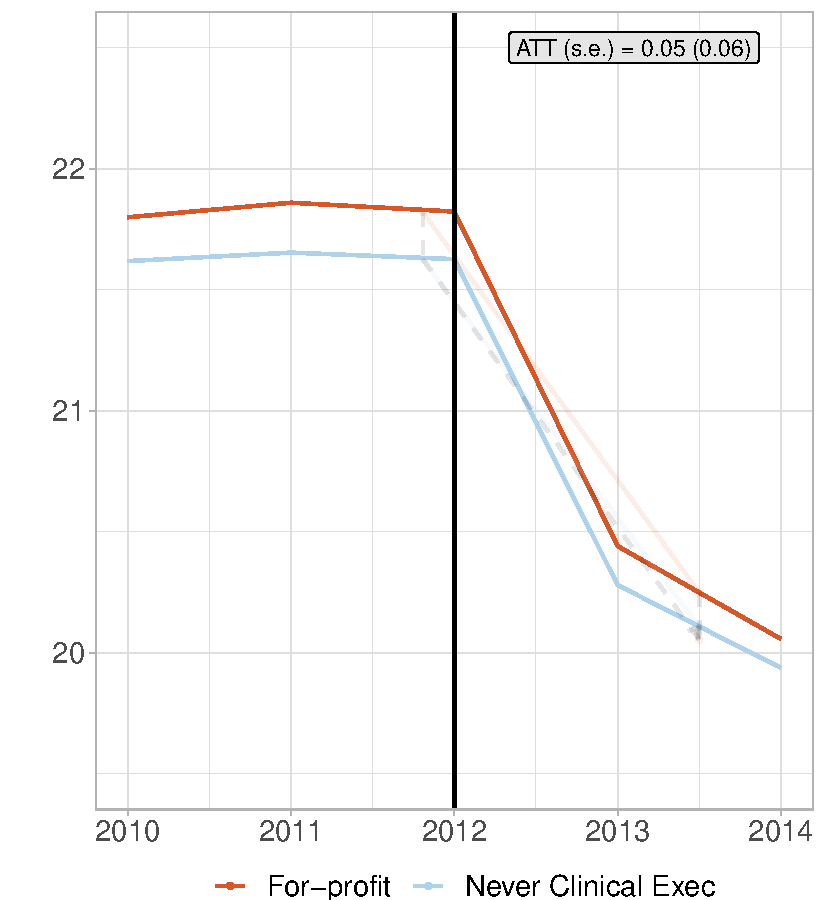
\includegraphics[width=\textwidth]{Objects/fp_read_nomd_synth_graph.pdf}
         \label{fig:read_synth_plotc}
     \end{subfigure}
        \label{fig:read_synth_plot}
    \end{figure}

    The estimates and graphical representation of the effect of being for-profit is shown in Figure \ref{fig:read_synth_plot}. In panel \ref{fig:read_synth_plotb}, the average treatment effect shows the effect of being for-profit compared to nonprofit with clinical executives on readmission rates after pay-for-performance changes. While readmission rates trend similarly prior to the incentive change, for-profits decrease readmission rates by .3 more than nonprofits with clinically trained executives. That is, for-profits respond more aggressively to the incentive change than nonprofits with clinical leadership. This difference is nearly identical to the difference between clinical and non-clinical teams shown in Section \ref{sec:clinical}. So, unsurprisingly, panel \ref{fig:read_synth_plotc} shows no such difference when comparing for-profits to nonprofits without clinically trained executives. Not only is the estimate not statistically significant, but the magnitude indicates a precise zero. That is, a lack of clinically trained executives leads nonprofits to act like for-profits in terms of readmission rates when responding to this incentive change. 

    Next, I present estimated differences in mortality rates between different hospital types in Figure \ref{fig:mort_synth_plot}. In panel \ref{fig:mort_synth_plotb}, the estimated difference is between for-profits and nonprofits with clinically trained executives. The magnitude of the difference in mortality rates is .08, where clinical team hospitals continue on an increasing trend and for-profits remain stable in mortality rate. While I cannot rule out a lack of differential response, the documented noisiness of mortality measures (\cite{mackenzie2016measuring}) may mean that the true effect is different from zero. However, the estimated difference in mortality between for-profits and nonprofits without clinically trained executives is certainly zero with a amgnitude of .03, shown in panel \ref{fig:mort_synth_plotc}.  


    \begin{figure}[ht!]
     \caption{Comparison to For-Profit: Mortality}
     \centering
     \begin{subfigure}[b]{0.45\textwidth}
         \centering
         \caption{For-Profit and Always Clinical Exec}
         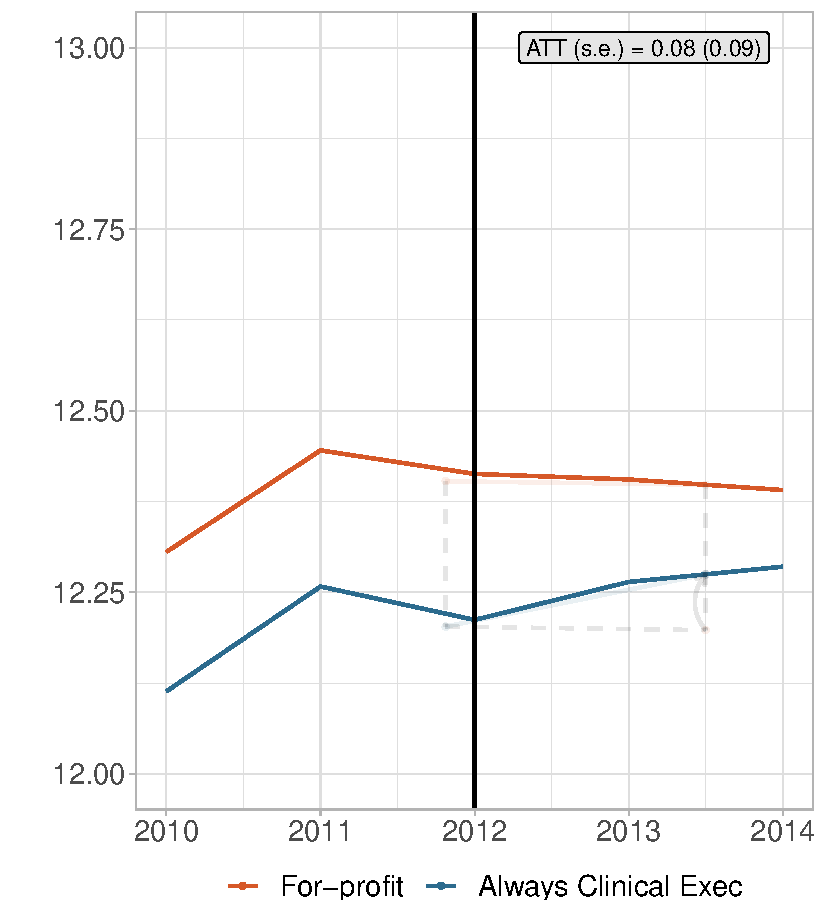
\includegraphics[width=\textwidth]{Objects/fp_mort_md_synth_graph.pdf}
         \label{fig:mort_synth_plotb}
     \end{subfigure}%
     \hfill
     \begin{subfigure}[b]{0.45\textwidth}
         \centering
         \caption{For-Profit and Never Clinical Exec}
         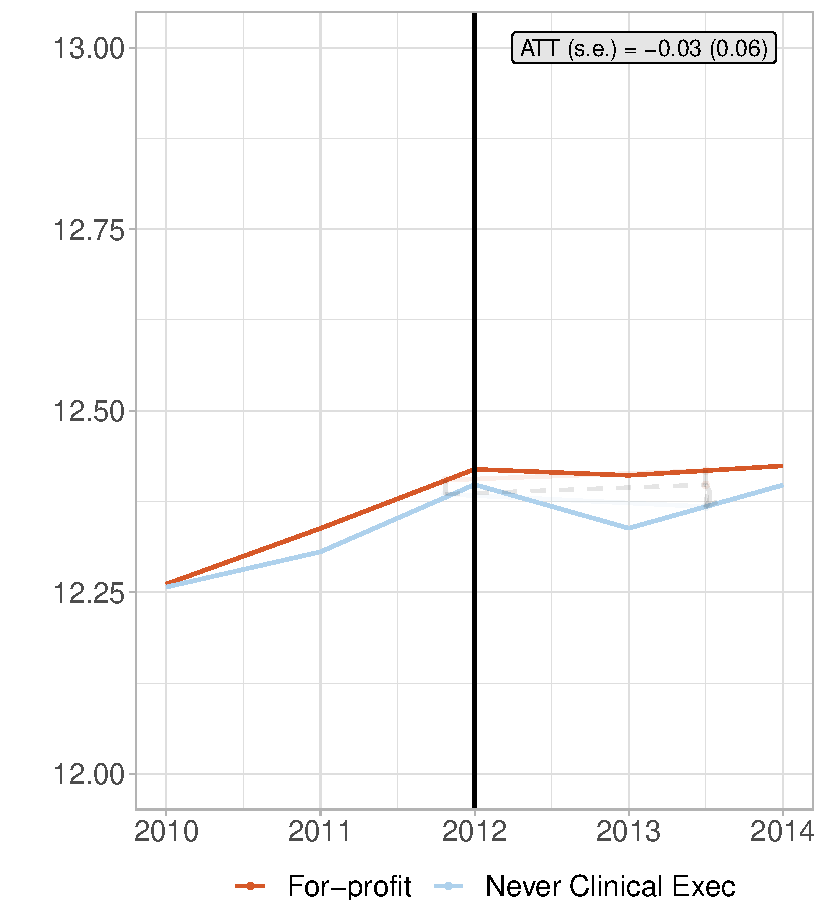
\includegraphics[width=\textwidth]{Objects/fp_mort_nomd_synth_graph.pdf}
         \label{fig:mort_synth_plotc}
     \end{subfigure}
        \label{fig:mort_synth_plot}
    \end{figure}
    

\section{Signaling vs. Managing Decomposition}\label{sec:sig_man}

    Given that having clinically trained executives affects behavior, an important distinction is whether the existing clinical leaders \textit{reveal} the underlying objectives of the hospital, or \textit{manage} the hospital differently. Up to this point, I have limited the sample of nonprofit hospitals to those that don't change their propensity to hire a clinically trained executive over the sample period, which combines any signaling and managing effects. However, under the assumption that hiring or firing these types of executives is not correlated with the pay-for-performance policy changes, such changes can be leveraged to decompose the effect into signaling versus managing. Therefore, I first investigate leadership changes in response to the policy change. 

    \subsection{Leadership Change Analysis} \label{sec:changes}

    I have discussed the assumptions of parallel trends, no anticipation, and no other confounding events in both Sections \ref{sec:clinical} and \ref{sec:forprofit}. These assumptions are also necessary here. Further, this decomposition analysis depends heavily on leadership team changes not endogenously occurring due to pay-for-performance policies. Up to this point, that assumption was important because of the way I selected the sample. However, this decomposition depends directly on leveraging such leadership changes. Thus, I now explore this assumption in detail. First, I present raw means over time that represent the fraction of hospitals who hire a clinical executive, fire a clinical executive, or have any change in their propensity to have a clinical executive in Figure \ref{fig:change_means}. There do not seem to be any drastic changes in 2011 or 2012 when the policies were becoming relevant to hospitals. 

    \begin{figure}[ht!]
    \centering
    \caption{Leadership Change Means Over Time}
    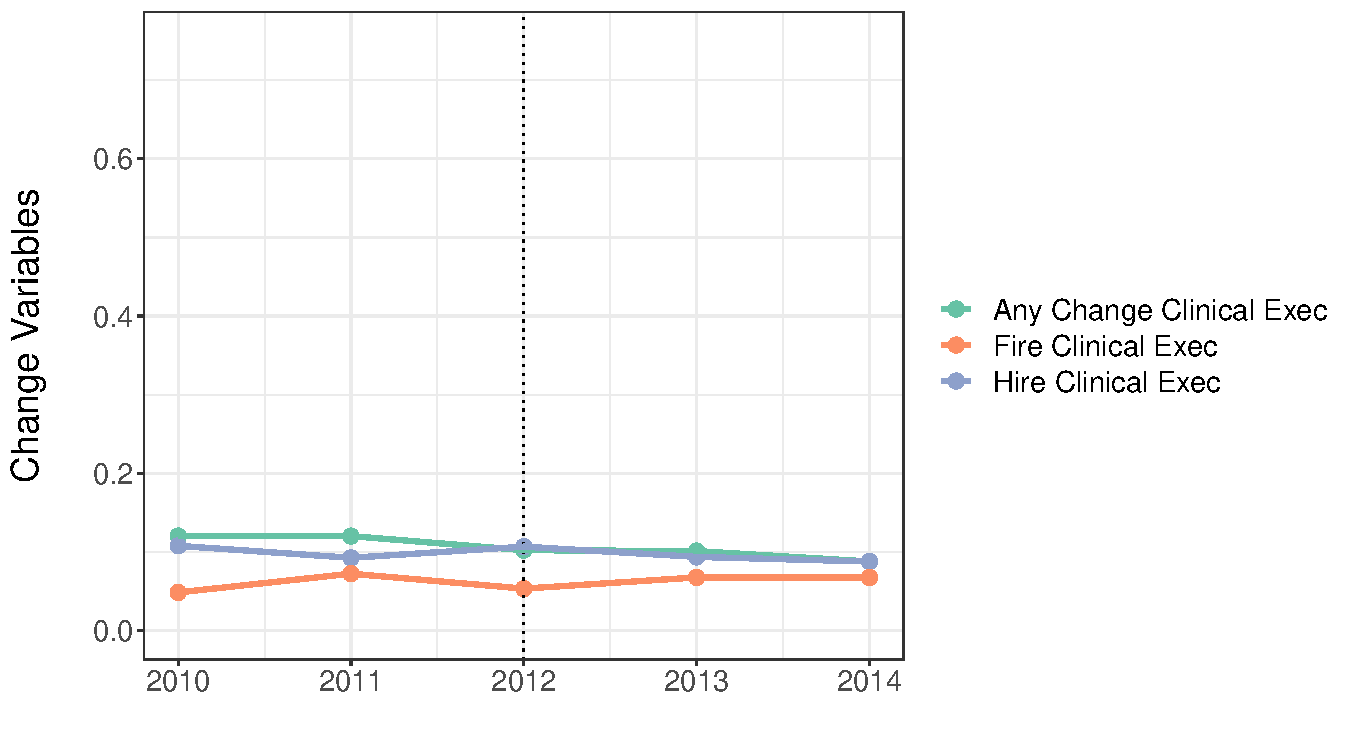
\includegraphics[width=0.8\textwidth]{Objects/change_means.pdf}
    \label{fig:change_means}
     \end{figure}

    Next, I assess whether this assumption is reasonable by analyzing how executive team changes are occurring over time for certain groups of hospitals. I estimate:

    \begin{equation}\label{eq:change2}
    \text{change}_{ht} = \sum_{j=2011}^{2014}\beta_j(\mathbf{1}\{t=j\}\times \text{Program Exposed})_{ht} + \alpha_h + \epsilon_{ht},
    \end{equation}

    where the variable $\text{Program Exposed}_{h}$ has three definitions. First, an indicator for whether the hospital was ever penalized under HRRP. Second, an indicator for whether the hospital ever received payments under HVBP. And finally, I leave out the Program Exposed variable to simply see how changes are correlated with given years for all hospitals. The outcome change$_{ht}$ is an indicator for whether the hospital changes the number of clinical executives in a given year. The estimates from this analysis are presented in Figure \ref{fig:change_analysis}. All estimates are not statistically different from zero, indicating that expectations of program exposure do not lead to changes in propensity to hire a clinical executive. Thus, it seems unlikely that endogenous team formation is biasing the estimates. 

     \begin{figure}[ht!]
         \centering
         \caption{Leadership Analysis Results}
         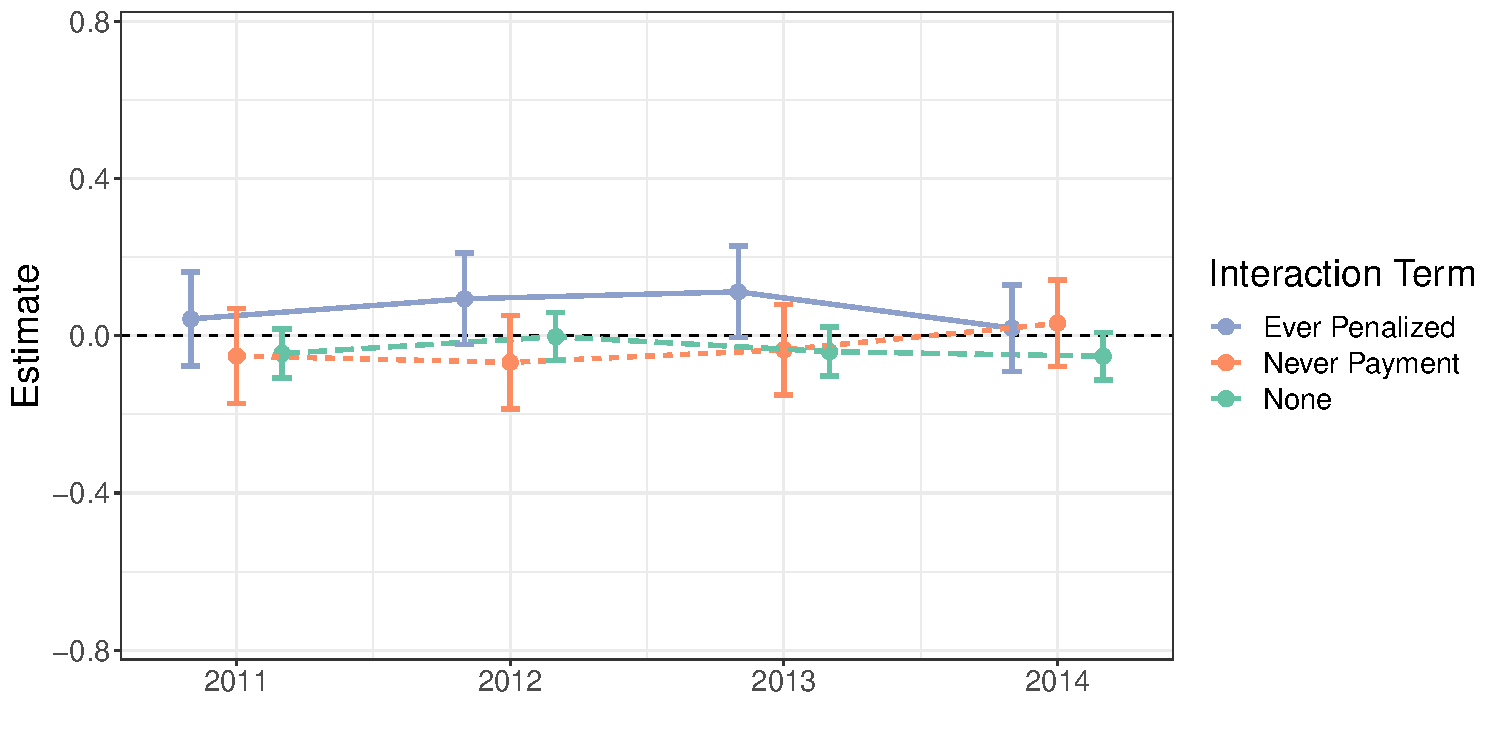
\includegraphics[width=0.8\textwidth]{Objects/change_analysis_plot.pdf}
         \label{fig:change_analysis}
     \end{figure}

     \subsection{Estimation}

    To disentangle the two, I carefully define the ``treat" and comparison group of hospitals in the following estimating equation. For clarity, I present the specification details in Figure \ref{fig:decomp_spec}. If clinically trained leaders are simply signals of underlying objectives, it shouldn't matter when hospitals have hired a clinical executive. For example, take two hypothetical hospitals. Hospital A has a clinically trained executive from 2010-2011. Hospital B has a clinical executive from 2010-2013. If clinically trained executives are a signal of underlying objectives, these two hospitals should respond similarly to pay-for-performance objectives despite only one of them having a clinical executive in 2012. However, if clinically trained leaders manage the hospital in a unique way, these two hospitals would respond differently since only one of them has clinical leadership in 2012 when the policy changes occurred. 

    \begin{equation}
    \label{eq:decomp}
    y_{ht} = \beta \text{ (treat x post 2012)}_{ht} + \gamma_{h} + \delta_t + \epsilon_{ht},
    \end{equation}

    Thus, in one specification I compare hospitals who ever have a clinically trained executive to hospitals who never have a clinically trained executive. This captures the signaling effect. In another specification, I remove all hospitals who never had a clinically trained executive, and compare hospitals who had a clinically trained executive in 2012 to those who had a clinically trained executive in any year except 2012, capturing a managing effect. 
    

\begin{figure}[ht!]
\begin{center}
\caption{\label{fig:decomp_spec}Decomposition Model Specification Details}
 
 \begin{tabular}{| m{18em} |}
 \hline
 Signaling:\\ [0.5ex]
 \hline\hline 
 \vspace{2mm}
 Treat Group:  \hspace{15mm} Never MD \\
 \vspace{2mm}
 Comparison Group: \hspace{3mm} Ever MD  \\
 [1ex]
 \hline
 \end{tabular}
\hfil   %<---
 \begin{tabular}{|m{18em}|}
 \hline
 Managing:\\ [0.5ex]
 \hline\hline
 \vspace{2mm}
 Treat Group: \hspace{11mm} No MD in 2012 \\
 \vspace{2mm}
 Comparison Group:  Ever MD (not in 2012)  \\
 [1ex]
 \hline
 \end{tabular}
 
\end{center}
 \end{figure}


    The estimates of each decomposition specification are shown in Table \ref{tab:MD_noMD_readmort_decomp_synth}. The readmission rate estimates are in columns (1) and (2), and mortality rate estimates are in columns (3) and (4). The first row compares ever clinical executive hospitals to never clinical executive hospitals, and the second row compares hospitals with a clinical executive in 2012 to hospitals who have a clinical executive in a year other than 2012. While there is no statistically significant estimate, the coefficients of the managing effect are very similar to the full effect found in Section \ref{sec:clinical}. The coefficients for the signaling effect are both statistically insignificant and close to zero in magnitude. Thus, I can rule out that clinical executives are simply a signal of underlying hospital objectives. 

    \import{Tables}{MD_noMD_readmort_decomp_synth.tex}


    \section{Conclusion}

    While previous literature has documented correlations between executive characteristics and firm behaviors/performance, research is still limited on this topic in the health care sector. This paper investigates whether having executive leaders with clinical training impacts hospital behaviors and outcomes, particularly in response to a policy change that financially incentivizes quality.I collect data on the names of hospital executives from 2010-2014 from publicly available Tax Form 990s, which are completed by all nonprofits in the US. I merge this data with existing hospital and physician characteristics, and aggregate to the hospital level. Thus, I utilize a unique data set of nonprofit US hospitals that captures the proportion of clinical executives, specialties of clinical executives, hospital characteristics, and hospital quality metric outcomes. 

    In 2012, two pay-for-performance policies went into effect that either penalized hospitals with high readmission rates, or gave payments to hospitals with low readmission/mortality rates. These policies were relevant to hospital finances, and gave tangible incentive for hospitals to increase quality. Thus, I leverage this exogenous policy change and estimate how clinically trained executives affect readmission and mortality rates in response to the change using a synthetic difference-in-differences strategy. Conditional on parallel trends holding, I find that having clinical experience mitigates the response to the incentive change. That is, while all hospitals reduce readmissions after the policies take place, non-clinical teams reduce readmissions at a fast rate than clinical teams. 
    
    I investigate several mechanisms by which this difference could occur. First, this result is not driven by non-clinical teams adjusting their patient complexity. However, comparing non-clinical teams to for-profit hospitals reveals that it could be underlying preferences for profit vs. patient benefit that drive the difference. Finally, I leverage exogenous changes in executive teams to show that clinically trained executives are not simply a signal of underlying preferences, but manage the hospital differently. 

    These findings have significant policy implications, as it informs the way different types of hospital leadership respond to policy changes. While I do not directly estimate the effect of hiring a clinically trained executive, I do show evidence that clinically trained executives on average place higher value on patient care. Thus, another way to incentivize quality is to encourage clinical leadership. 

    

	
	\newpage

    \printbibliography

\appendix

 \section{Data}\label{appendixdata}

\subsection{Gathering Hospital Leadership Names}

I use the Nonprofit Explorer API to access the archive of NFP tax form 990s. At the time of writing this, information on using version 2 of the API can be found at \hyperlink{https://projects.propublica.org/not-for-profits/api}{https://projects.propublica.org/not-for-profits/api}. 
    
There are over 1.5 million not-for-profit entities in the US, making it crucially important to be able to filter by type of entity before analyzing any PDFs. The API allows this by filtering a query based on National Taxonomy of Exempt Entities (NTEE) code. I query only not-for-profits categorized as E20 (hospitals), E21 (community health systems), and E22 (general hospitals). The API has a pagination limit of 100, meaning I can only pull information on 100 hospitals at a time. Therefore, I filter the query further to only consider one state at a time. The only state that has more than 100 entities registered is California, and thus I subset the California query even further by names that include the word "hospital" and names that don't. I combine all of these subsets and have information on each not-for-profits Employee Identification Number. There are 5,588 EINs total in this list. This acts as a list of entities for which I can pull more information. 

I loop through the list of EINs found in the previous step and query more detailed information from the API on that specific EIN. I save the name, secondary name, state, and zip code, all of which do not vary by year. I also save each year's URL link to the Tax Form 990 PDF. For the sake of a comprehensive data set, I keep years 2006-2020 (I later limit to 2010-2014 when focusing on pay-for-performance initiatives in 2012). Thus, I finish this step with a panel data set of EIN characteristics and PDF locations. Importantly, there are multiple types of Tax Form 990s depending on the size of the not-for-profit. In many cases, one not-for-profit has at least two different forms filed in a given year. I filter out any EIN-years for which there are no PDFs on file. The data on PDF locations contains 4,012 EINs and 61,363 EIN-year-tax forms.

It is necessary to link these not-for-profits with other sources of data to recover penalties from HRRP, payments from HVBP, bed size, and outcomes of interest. The ideal hospital data set to match to is American Hospital Association (AHA) Survey, which contains hospital characteristics and Medicare ID number. However, an EIN to AHA ID crosswalk does not exist. Therefore, I take a conservative approach to matching EINs to American Hospital Association (AHA) ID based on hospital name and location. First, I will discuss limitations and cleaning of the AHA data and tax form data. 

In the AHA data, I filter only to hospitals in the contiguous US, Alaska, and Hawaii (excluding places like Puerto Rico), classified as not-for-profit or state/community, and those that are general acute care. I also filter out any hospitals who weren't present in the data (or change system ID) in 2009-2015, meaning they either closed or were acquired. Due to the survey nature of this data, a hospital name may look slightly different from one year to the next. For example, ``Waldo County General Hospital" is also ``Waldo County General Hospital Maine Health". Further, zip codes may change by one or two digits, making them unreliable to match based on. To deal with this, I first keep only unique AHA ID, name, zip, state, and system name combinations. Then, I convert the data from long to wide so that each AHA ID occurs only once, but may have multiple names, zip codes, or system names associated with it.

I consider which not-for-profit entities are not likely to be hospitals and drop them. There are numerous foundations or auxiliary firms with the purpose of raising funds for the hospital, but do not provide services to patients. I filter out any not-for-profit with "foundation" or "auxiliary" in the name. I also filter out various specialty centers that fell into the general hospital category, such as hospice or cancer centers. 

I then proceed matching based on names in multiple layers. I focus on exact string matches, so I remove all spaces and common characters that could cause mismatches such as \&, ', -, and inc. Next, I take each AHA name and look for exact matches in a not-for-profit's first or secondary name for not-for-profits in the same state as the AHA hospital. When an exact match is found, I record the link between AHA ID and EIN. In this first layer of matching, 860 hospitals in the AHA data are linked to an EIN, equivalent to 31\% of AHA not-for-profit hospitals in the sample. 

In the next layer of matching, I remove common words such as "healthcare", "regional", "hospital", etc. That way if there are subtle differences in names, removing common words may allow for an exact match. Again, I take each AHA hospital name and look for exact matches in the not-for-profits within the same state. This adds an additional 90 hospital matches, accounting for a total of 34.5\% of AHA hospitals. Finally, I manually search through unmatched EINs to identify any matches. From google searches, I identify an additional 300 EIN-AHA ID matches.

I then extract the names of board members and executives from the Tax Form 990 PDFs of matched hospitals. In the data set of hospital PDF URLs that I collected earlier, I limit to the hospitals with solid matches described above. I then loop through each EIN, downloading PDFs locally and using the tesseract package in R to extract text from the relevant pages of the PDF using OCR text extraction methods. In particular, I loop through each page of the PDF, look for the title associated with leadership names: ``Officers, Directors, Trustees, Key Employees, and Highest Compensated Employees", and save all the text from any pages where this title is found. I save the text to a list of all EIN, years present. 

One tricky aspect of the NonProfit Explorer API is that, only in some cases, if two forms are present for an EIN, year, only the first one (which is typically not the one with the relevant information) is pulled. Therefore, for some hospitals, a couple years will have gaps in text extraction data. I locate EIN, years where this problem is occurring, and a team of RAs locates and downloads the correct forms manually. I extract text from these manually downloaded forms in the same manner as above. 

The form of the text data is a data frame with one column, where each line of text is saved in a different row. Typically on the same page as the names and positions is a list of the highest compensated employees and their compensation. In order to not record extra names, I filter out any rows after the start of this section. I then remove any digits, parentheses and brackets, other punctuation, letters that occur by themselves, two letter ``words" that have no meaning, and excess space between words. I then split up the phrase into individual words, so one phrase with 5 words is broken up into 5 variables. I write a text cleaning function that locates names, positions, titles, and indications of resigning. I flag name rows using the Census name list data for the year 2000. The columns with the most flags are then identified as name columns. I then extract any text that indicates a doctor title and link it to the name located the closest to it. Similarly, I extract text of all potential positions such as CEO, CFO, CMO, president, board member, etc., and link it to the name most closely located to it. 

I then create a name-level data set that only includes executives. That is, I remove all board members from the data. I then create hospital level indicators based on the names, titles and positions associated with the hospital: the number of MD executives, the number of total executives, and whether the hospital employs a CMO. In Figure \ref{fig:state_doc}, I show the percent of hospitals with a clinical executive in each state. This figure verifies that clinical executives are not concentrated in a small region geographically. 

\begin{figure}[ht!]
    \centering
    \caption{Percent of Hospitals with Clinical Executives by State}
    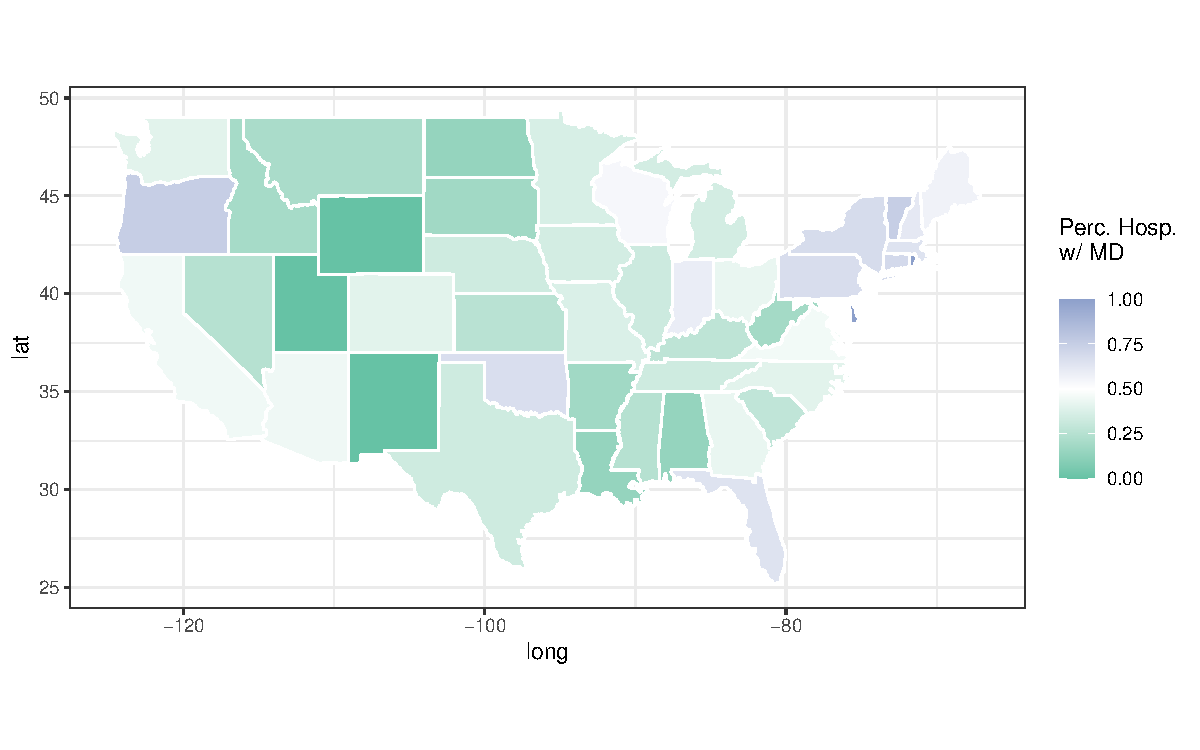
\includegraphics[width=\textwidth]{Objects/has_doc_avg_map.pdf}
    \label{fig:state_doc}
\end{figure}

\section{Additional Summary Statistics}\label{app:sumstats}

\import{Tables}{forprofit_sample_sumstats.tex}

\subsection{Matched vs. Unmatched Not-for-Profits}\label{app:matched}

The sample of all NFP hospitals that I use for analysis consists of 852 hospitals. In the AHA data, there are 2,258 additional NFP hospitals that either were not matched to tax forms, did not exist in the tax form data, or did not have executive names in the tax forms. While it would be ideal to analyze all NFPs, a sample size of 852 firms is relatively large in the hospital executive literature. 

In this section, I compare the in-sample NFPs to the out-of-sample NFPs along observable measures. I present means and standard deviations of these measures in Table \ref{tab:nfp_sample_compare}. The in-sample NFPs are slightly larger in terms of beds and patients seen. They are also slightly more likely to be penalized or receive payments under the pay-for-performance incentives. However, average readmission and mortality rates are very similar, as well as case mix index. The largest difference in the two samples is that I under-represent NFP hospitals in systems. This is due to the nature of the tax form 990s, where systems often file one tax form for the entire system, making it difficult to discern the true managers of a specific hospital. Because of this, I drop hospitals from the sample who only have leadership information from a system tax form. 

\import{Tables}{NFP_sample_comparison.tex}

\subsection{Executive Team Changes}\label{app:changes}

I present the number of hospitals who change their propensity to hire a clinically trained executive at different times in Table \ref{tab:change_timing}. I break the timing up into pre-2012, 2012, and post-2012. I show the number of hospitals who have MDs in different time combinations. The number of hospitals that only have an MD executive in 2012, but at no other time, is only 6. The majority of hospitals (187) who ever have a clinical executive have one in every time period. 

\import{Tables}{change_num_table_2012.tex}


\section{Modeling Hospital Response to Pay-for-Performance}\label{sec:model}

    I model hospital behavior under two simplified worlds: one where quality does not directly affect profit, and one where it does. Pay-for-performance incentives essentially incorporate performance directly into a hospital's profit function (\cite{dranove2011health}). I directly model performance as quality of care, which is inversely related to readmission and mortality rates. While the literature speculates about the true form of NFP objective functions, we can generally think of hospitals choosing some linear combination of profit and societal benefit, without knowing how much weight the hospital places on each. Intuitively, a hospital that places only weight on profit (for-profit type) will only care about quality when it enters into the profit function, and therefore will respond more drastically to pay-for-performance than a hospital who already cared about quality through societal benefit before the incentives. Therefore, hospital responses to pay-for-performance incentives reveal information about their underlying preference on profit vs. societal outcomes. 

    To formalize this intuition, I specify the hospital objective function as a weighted average of profit and societal (or patient) outcomes and derive characteristics of the optimal quality. For simplicity, I abstract away from quality having a direct effect of quantity and price. Without any financial incentives to increase quality, hospital quality is decided by:  
    
    $$\max_{\theta}\hspace{2mm}\alpha\left[R - c_{\theta}(\theta) \right] + (1-\alpha) u(\theta),$$

    \noindent where $R$ is net revenue, $c_{\theta}(.)$ is an increasing cost function specific to quality $\theta$, $u(.)$ is extra utility gained from quality, which is increasing and concave in $\theta$, and $\alpha\in[0,1]$ captures the weight placed on profit vs. societal benefit. There is an implicit stay-open condition throughout the model. Taking the first order condition yields 

    $$(1-\alpha)u'(\theta) = \alpha c_{\theta}'(\theta),$$

    \noindent where marginal benefit equals marginal cost of increasing quality. Solving for $u'(\theta)$ and differentiating with respect to $\alpha$:

    $$\frac{du'(\theta)}{d\alpha} = \frac{1}{(1-\alpha)^2}c_{\theta}'(\theta) > 0.$$

    \noindent Thus, by the Implicit Function Theorem, 

    $$\frac{d\theta}{d\alpha} = \frac{du'(\theta)/d\alpha}{du'(\theta)/d\theta} < 0.$$

    \noindent That is, the more weight on profit, the lower quality of care chosen by the hospital.

    In a world with pay-for-performance incentives, which can either look like benefits from high quality (such as HVBP) or penalties for low quality (as in HRRP), quality directly affects revenue. Thus, $R(\theta)$ is an increasing function of $\theta$, and I assume that the marginal financial benefit of increasing quality is greater than the marginal cost ($R'(\theta)\geq c_{\theta}'(\theta))$. Thus, the new first order condition yields:

    $$u'(\theta) = \frac{\alpha}{1-\alpha} \left[c_{\theta}'(\theta)-R(\theta)\right] \leq 0.$$

    \noindent Taking the derivative of this with respect to $\alpha$,

    $$\frac{du'(\theta)}{d\alpha} = \frac{1}{(1-\alpha)^2}c_{\theta}'(\theta).$$

    Therefore, again using the Implicit Function Theorem,

    $$\frac{d\theta}{d\alpha} = \frac{du'(\theta)/d\alpha}{du'(\theta)/d\theta}\geq0.$$

    That is, all else equal, in a world with financial incentives on quality, quality is increasing with more weight placed on profit. I combine the results found in each scenario into one response function that depends on $\alpha$, where $\theta_2$ is quality under pay-for-performance incentives and $\theta_1$ is quality with no financial incentive to quality. That is, 

    \begin{align*}
        \frac{d\Delta\theta}{d\alpha}&=\frac{d(\theta_2-\theta_1)}{d\alpha}\\
        &=\frac{d\theta_2}{d\alpha}-\frac{d\theta_1}{d\alpha}\\
        &\geq 0.
    \end{align*}


    Hence, this model predicts that change in quality depends on how much weight the hospital places on profit vs. societal benefit. Particularly, hospitals with more weight on profit respond more than hospitals with more weight placed on societal benefit. In reality, $\alpha$ is unknown, except in the case of for-profits, who have revealed that they have a high $\alpha$ by their ownership status. However, not-for-profit behavior on average does not bring much clarity about their objectives. An observable and economically relevant characteristic of a hospital that could affect $\alpha$ is composition of their executive leadership team. Thus, I compare the response of for-profits and not-for-profits with different leadership teams to bring clarity on how this might point to underlying $\alpha$.


\section{Results By Condition}\label{app:condition}


\import{Tables}{MD_noMD_readmort_condition_synth.tex}

\section{TWFE Regression and Event Study Results}\label{app:fullsample}

While I ultimately employ a synthetic difference-in-differences framework, I also present the coefficient estimates and event study tables under a typical TWFE model specification. That is, there is no weighting of the control group or time periods. Table \ref{tab:forprofit_readmort_fullsample} shows coefficient estimates for the three specifications under Equation \ref{eq:forprofit}. Columns (1)-(3) show coefficient estimates for the weighted average readmission rate outcome, and columns (4)-(6) show coefficient estimates from the weighted average mortality outcome. Generally, these results are qualitatively identical to the synthetic difference-in-difference specification results. There is a statistically significant difference in readmission rate response between for-profits and NFPs with a clinical executive. Specifically, for-profits decrease their readmission rates by .4ppts more than NFPs with a clinical executive. There is no difference (statistically or in magnitude) between readmission rate responses of for-profits compared to all NFPs and NFPs without clincal executives. 

Similarly to the synthetic diff-in-diff estimates, there is no statistical difference in mortality between any of the hospital types, but the magnitude difference between for-profits and NFPs with clinical executives is much larger. This oculd be due to the noisiness of mortality as a measure. 

\import{Tables}{forprofit_readmort_fullsample.tex}

Further, I present coefficient estimates in Table \ref{tab:MD_noMD_readmort_fullsample} directly comparing NFPs with and without clinical executives for both readmission and mortality rates. Again, these results are very similar to the main results of the paper, with only slightly larger magnitudes. NFPs without a clinical executive respond to the pay-for-performance incentives by decreasing readmission and mortality rates more aggressively than NFPs with clinical executives. 

\import{Tables}{MD_noMD_readmort_fullsample.tex}

Finally, I present these results in typical event study form in Figure \ref{fig:es_plot}, which show no evidence of significant pre-trends driving the findings. 

\begin{figure}[ht!]
     \caption{TWFE Event Study Results}
     \centering
          \begin{subfigure}[b]{0.45\textwidth}
         \centering
         \caption{}
         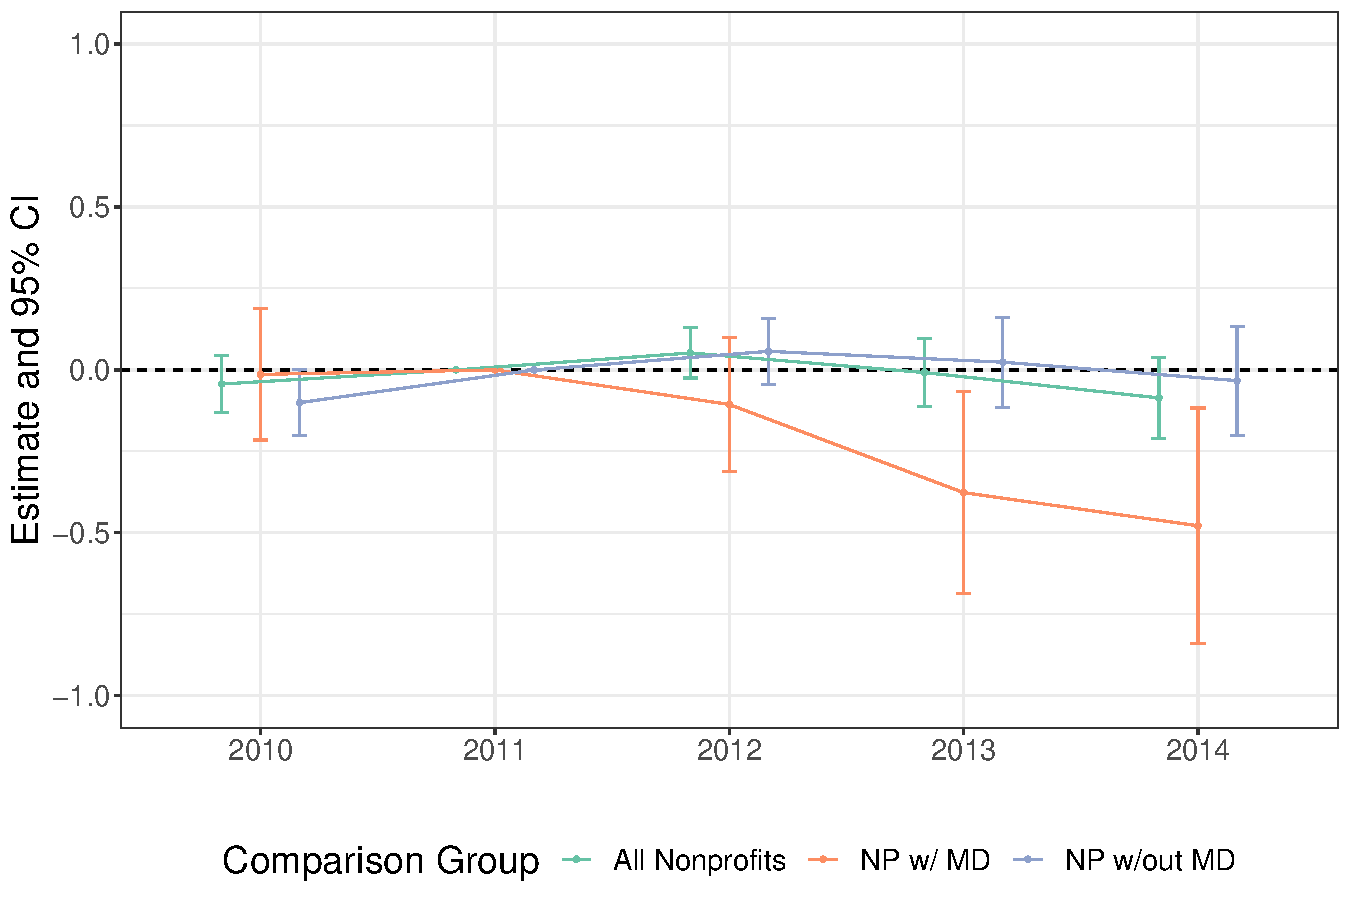
\includegraphics[width=\textwidth]{Objects/read_forprofit_es_graph.pdf}
         \label{fig:es_plota}
     \end{subfigure}%
     \hfill
     \begin{subfigure}[b]{0.45\textwidth}
         \centering
         \caption{}
         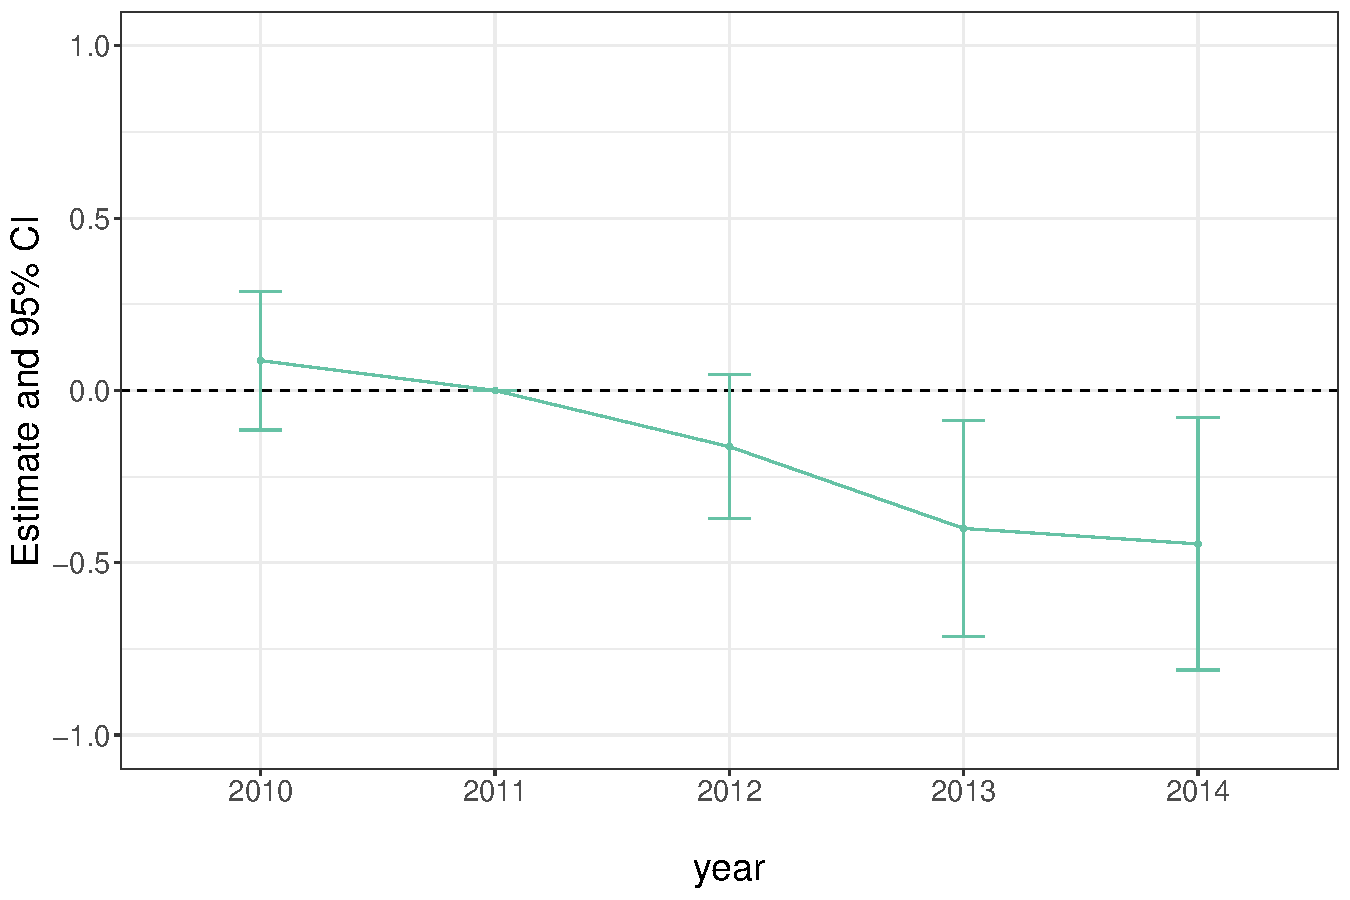
\includegraphics[width=\textwidth]{Objects/read_MD_es_graph.pdf}
         \label{fig:es_plotb}
     \end{subfigure}%
     \vspace{5mm}
     \hfill
     \begin{subfigure}[b]{0.45\textwidth}
         \centering
         \caption{}
         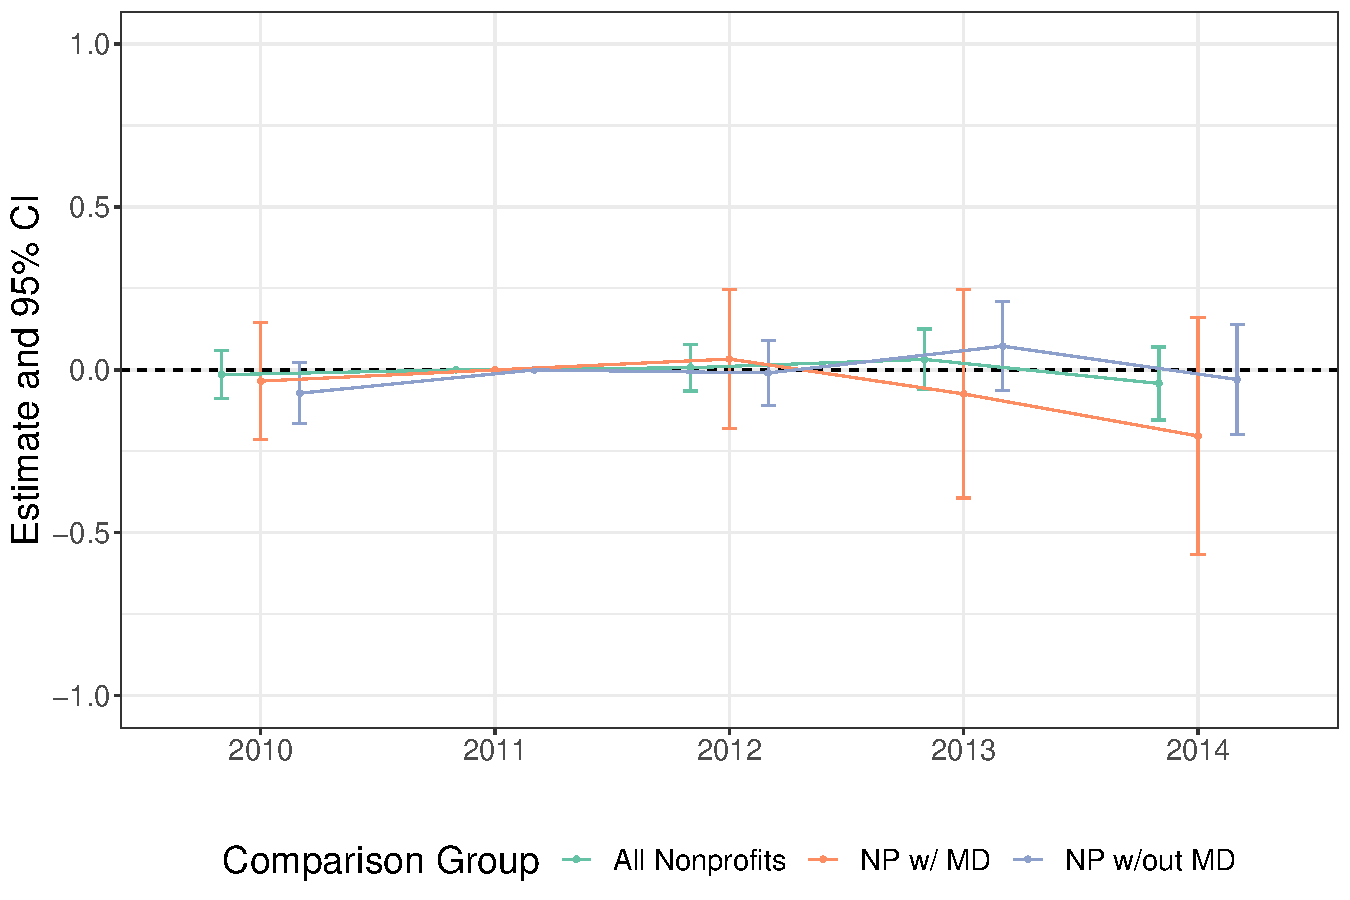
\includegraphics[width=\textwidth]{Objects/mort_forprofit_es_graph.pdf}
         \label{fig:es_plotc}
     \end{subfigure}
     \hfill
     \begin{subfigure}[b]{0.45\textwidth}
         \centering
         \caption{}
         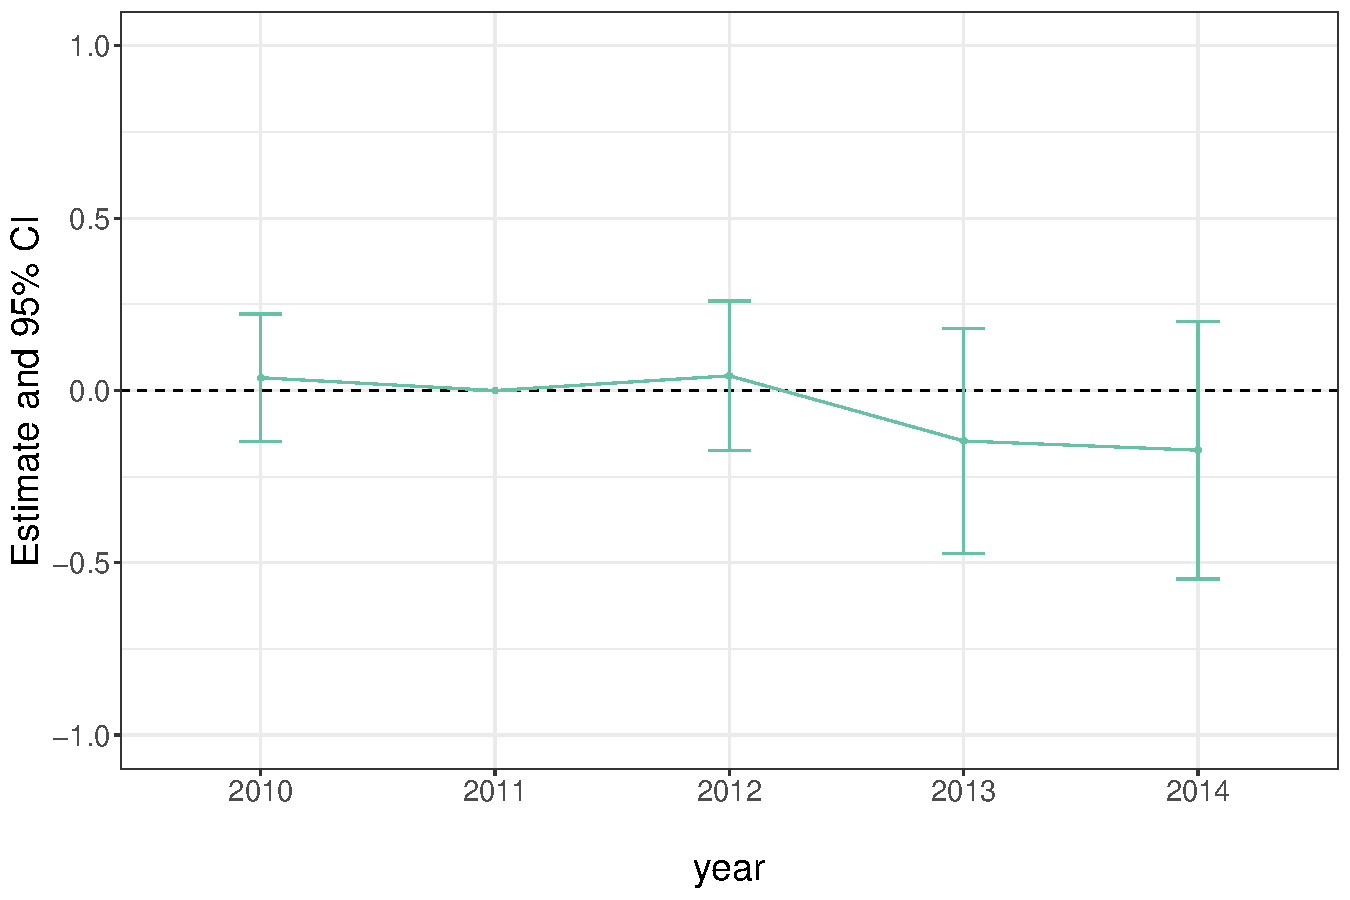
\includegraphics[width=\textwidth]{Objects/mort_MD_es_graph.pdf}
         \label{fig:es_plotd}
     \end{subfigure}
        \label{fig:es_plot}
    \end{figure}




\section{Synthetic Difference-in-Difference Coefficient Tables}

While I present the graphical representation of results in the main text, I also present a table of coefficients and standard errors for readmission and mortality rates in Tables \ref{tab:forprofit_readmort_synth} and \ref{tab:MD_noMD_readmort_synth}.

\import{Tables}{forprofit_readmort_synth.tex}

\import{Tables}{MD_noMD_readmort_synth.tex}


    

    

    

    

    

    

	
	
	


\end{document}

